\chapter{Correlative microscopy}

Combining multiple imaging techniques can provide insight into a specimen that would be difficult to obtain using a single technique.
However, this approach usually requires good surface preparation and accurate image registration.
This chapter shows workflows for different methods and demonstrates the possible benefits of correlative microscopy.


% \section{Combination of \acs*{SEM} - \acs*{BSE} + \acs*{EDX}}

% {\color{red} relevance? usually \ac{SEM} / \ac{BSE} + \ac{EDX} do already align - Measurements with ageing specimens/ retransferred specimens}

% \begin{enumerate}
%   \item realignement using fiducials
%   \item combination of \ac{SEM} - \ac{BSE} + \ac{EDX} + \ac{LAICPMS}
%   \item combination of \ac{SEM} - \ac{BSE} + µXRF
% \end{enumerate}



\section{Combination of \acs*{SEM} - \acs*{BSE} + \acs*{EDX} + \acs*{LAICPMS} }
\label{sec:corr_laicpms}

\textit{The results of this section are mostly published in \textcite{kleiner.2022b}. However, another area was chosen to discuss the results.}

The measurements were carried out on an embedded and polished clinker grain (composition, see \zcref{tab:phase-composition-clinker}).
They are visible as tiny dark spots (\zcref{fig:LAICPMS-specimen}), already indicating the damage induced by the laser ablation.
In total, there were three mapping areas and one spot analysis area, which is not evaluated in this work.

%\subsection{Example area}

The evaluation is described using one mapping position as an example.
\zcref{fig:LAICPMS-positon2} shows the area of the \ac{EDX} mapping and the subsequent \ac{LAICPMS} area on top of a \ac{BSE} image.

\begin{figure}[htb!]
  \centering

  \begin{subfigure}[t]{0.49\textwidth}
      \ifdefined\PRINTABLE
        \includegraphics[width=\linewidth]{la-icp-ms/position2.pdf}
      \else
        \animategraphics[loop,autoplay,width=\linewidth]{.5}{figures/la-icp-ms/position2-anim/Animation}{0}{4}
      \fi
    \caption{Data positioning}
    \label{fig:LAICPMS-positions}
  \end{subfigure}
  \hfill
  \begin{subfigure}[t]{0.49\textwidth}
    \includegraphics[width=\textwidth]{la-icp-ms/LA-BSE.pdf}
    \caption{\ac{BSE} image of the \ac{LAICPMS}-induced damage.}
    \label{fig:LAICPMS-site-damage}
  \end{subfigure}

  \caption{
    Position of the \ce{Si}-\ac{EDX}- ({\color{red}red}) and \ce{Ba}-\ac{LAICPMS}-mapping ({\color{orange}yellow}). \cite{kleiner.2021d}
  }
  \label{fig:LAICPMS-positon2}
\end{figure}

The areas measured contain all relevant phases, as \ac{C3S}, \ac{C2S}, \ac{C3A}, \ac{C4AF}, \ce{MgO}, \ce{CaO} and alkali sulphates.
\ac{C3S} and \ac{C2S} are easily identifiable in the \ac{BSE} image (\ac{C2S} appears a little darker than \ac{C3S}), but also in the \ac{EDX} mappings.
The \ce{Ca}, \ce{Si}, \ce{Al} and \ce{Fe} \ac{EDX} element distribution maps marked in \zcref{fig:LAICPMS-EDX}.

\begin{figure}[htb]
  \centering

  \begin{subfigure}[t]{0.32\textwidth}
    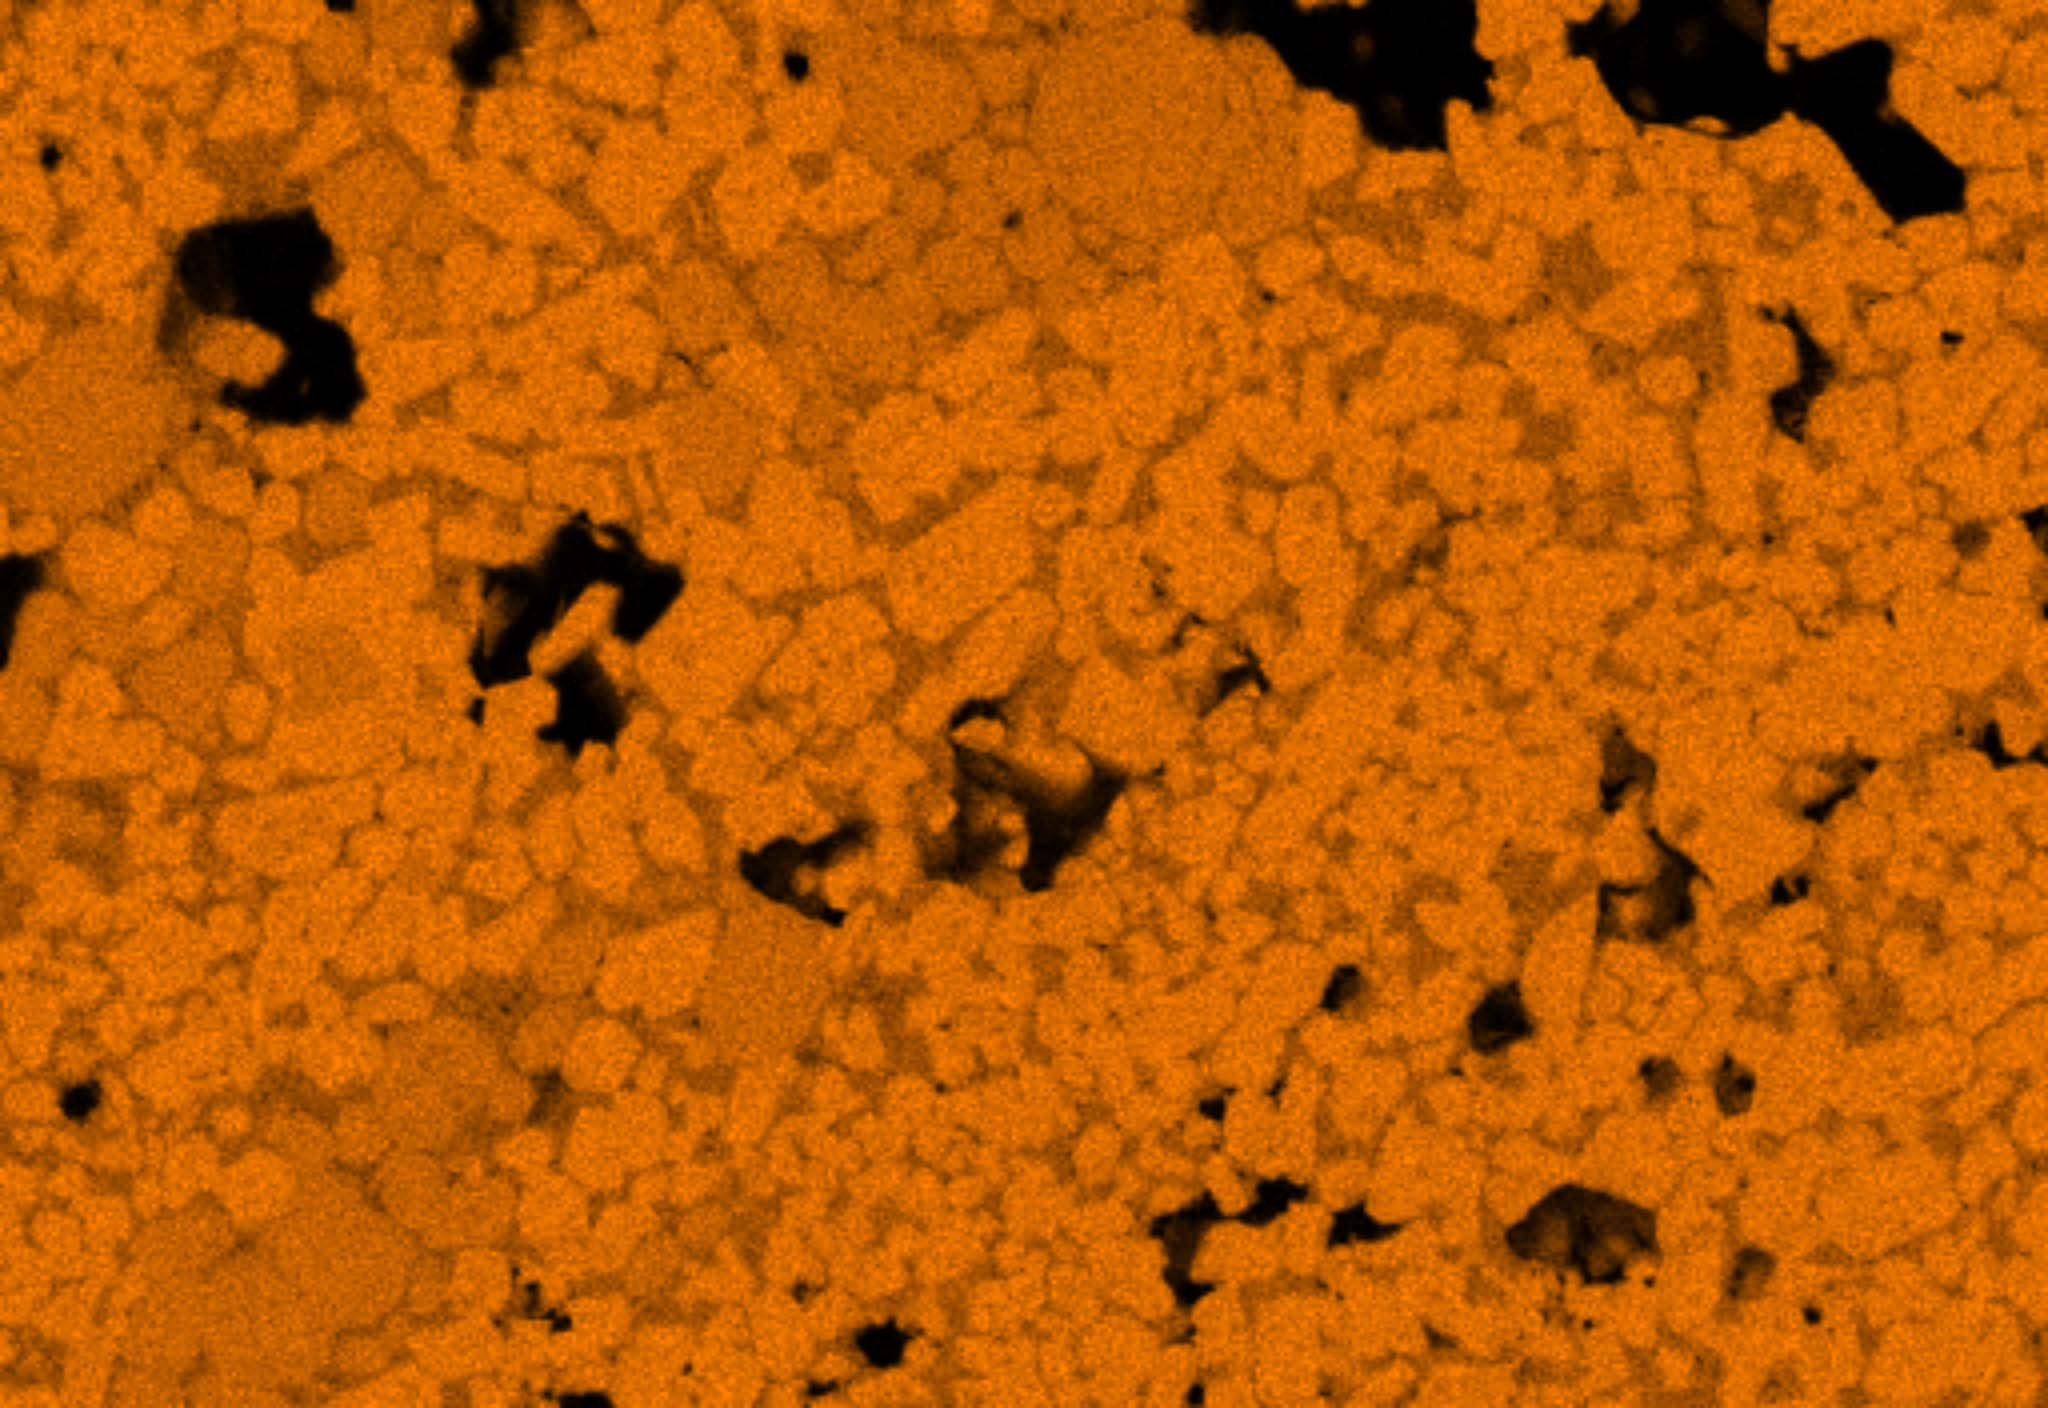
\includegraphics[width=\textwidth]{figures/la-icp-ms/edx/Ca.jpg}
    \caption{Ca mapping}
    \label{fig:LAICPMS-EDX-Ca}
  \end{subfigure}
  \hfill
  \begin{subfigure}[t]{0.32\textwidth}
    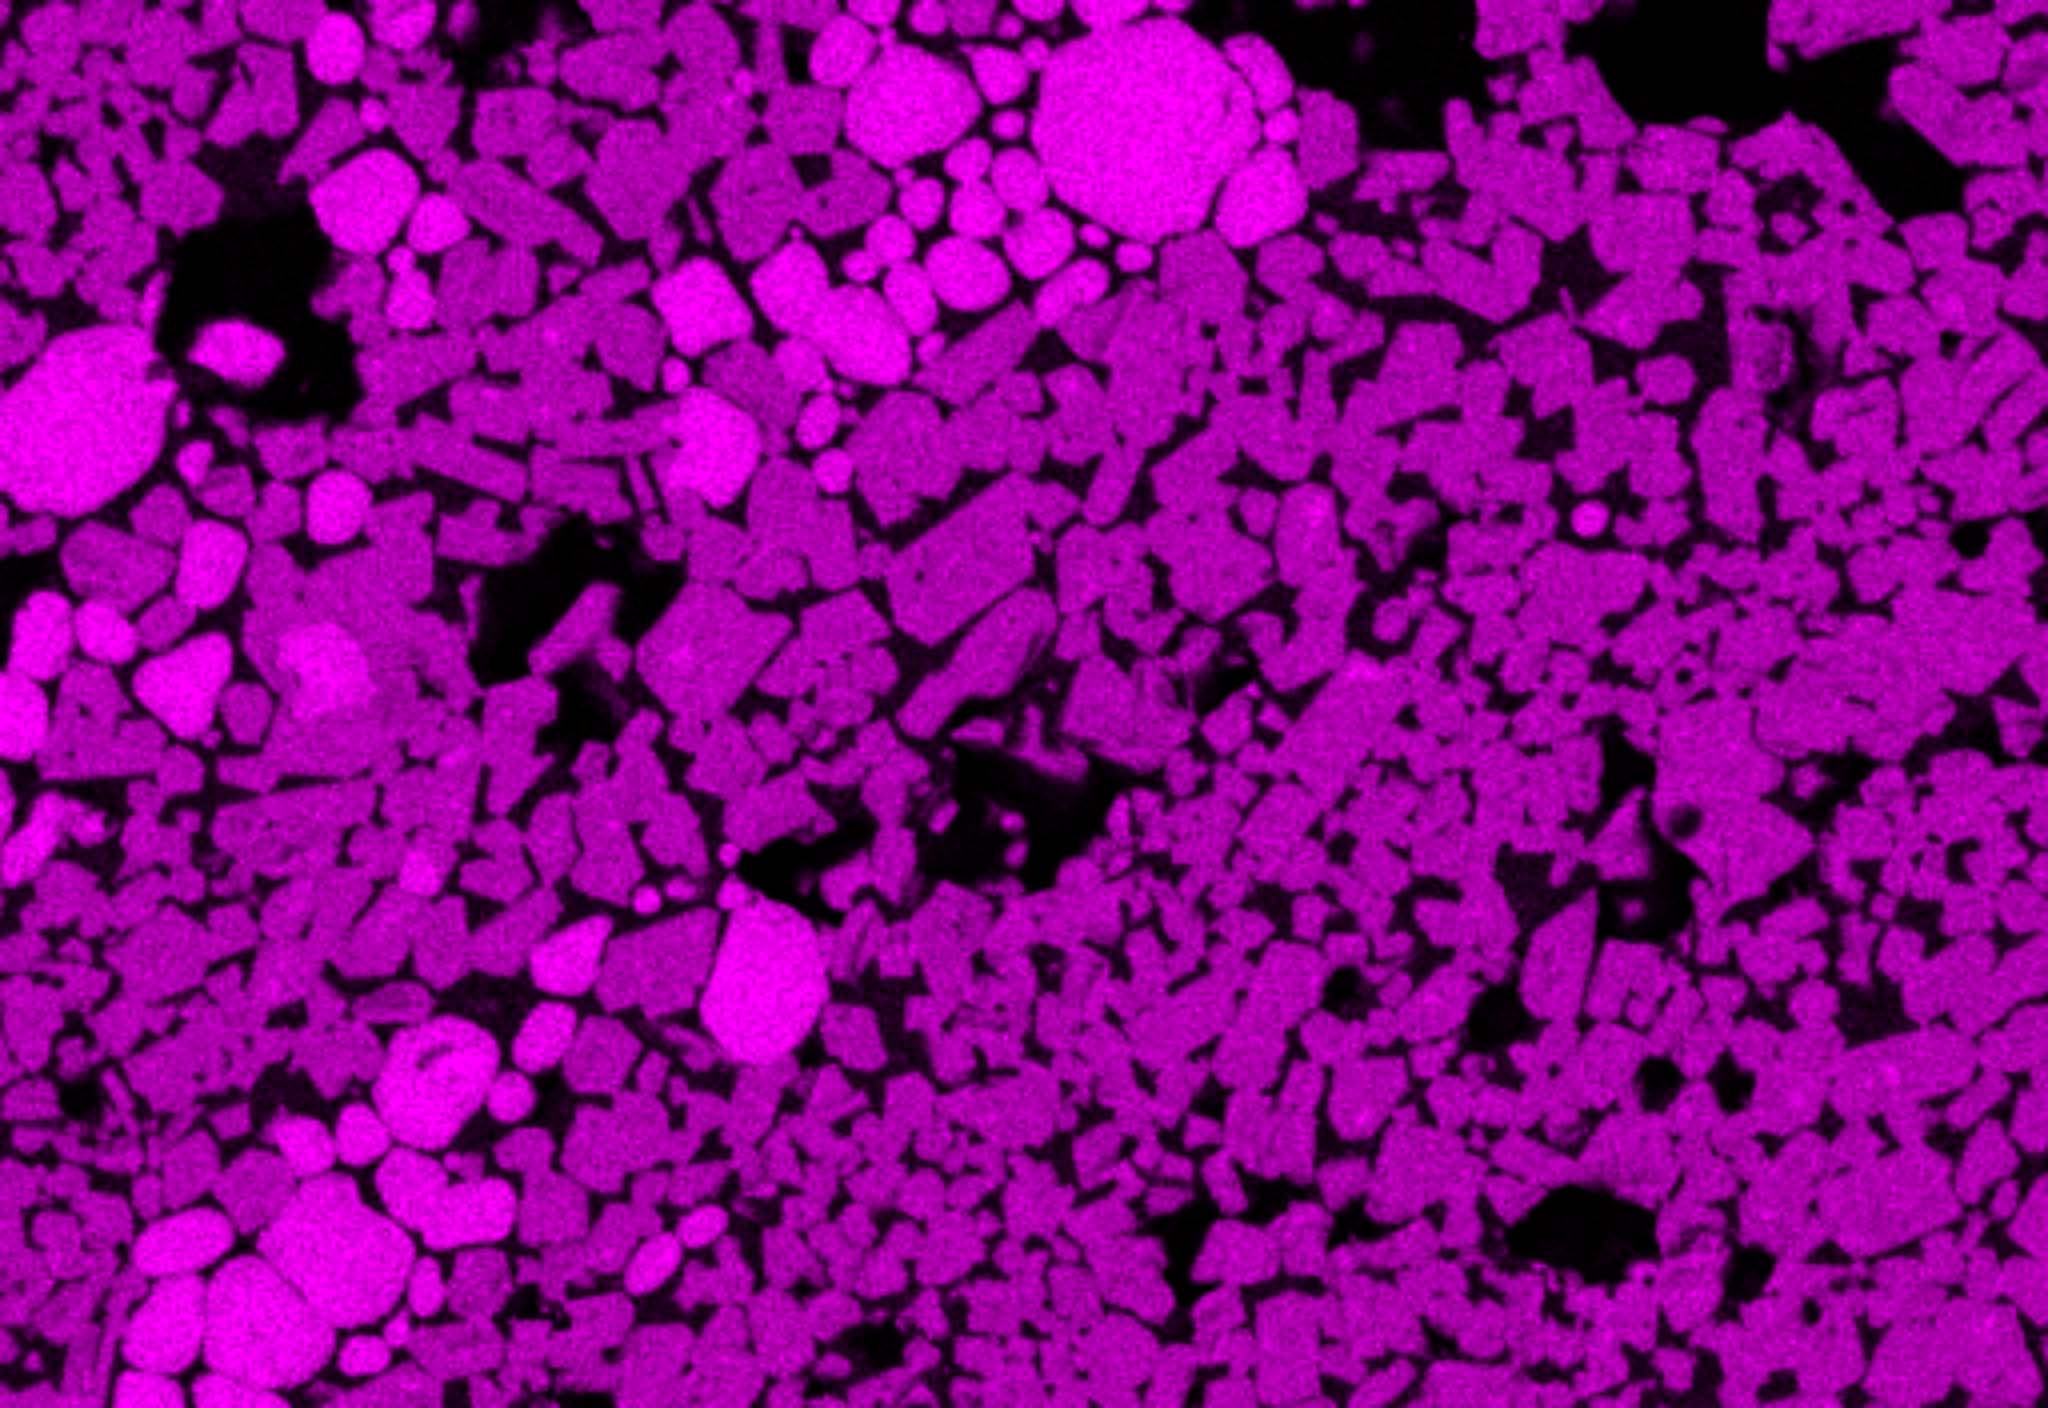
\includegraphics[width=\textwidth]{figures/la-icp-ms/edx/Si.jpg}
    \caption{Si mapping}
    \label{fig:LAICPMS-EDX-Si}
  \end{subfigure}
  \hfill
  \begin{subfigure}[t]{0.32\textwidth}
    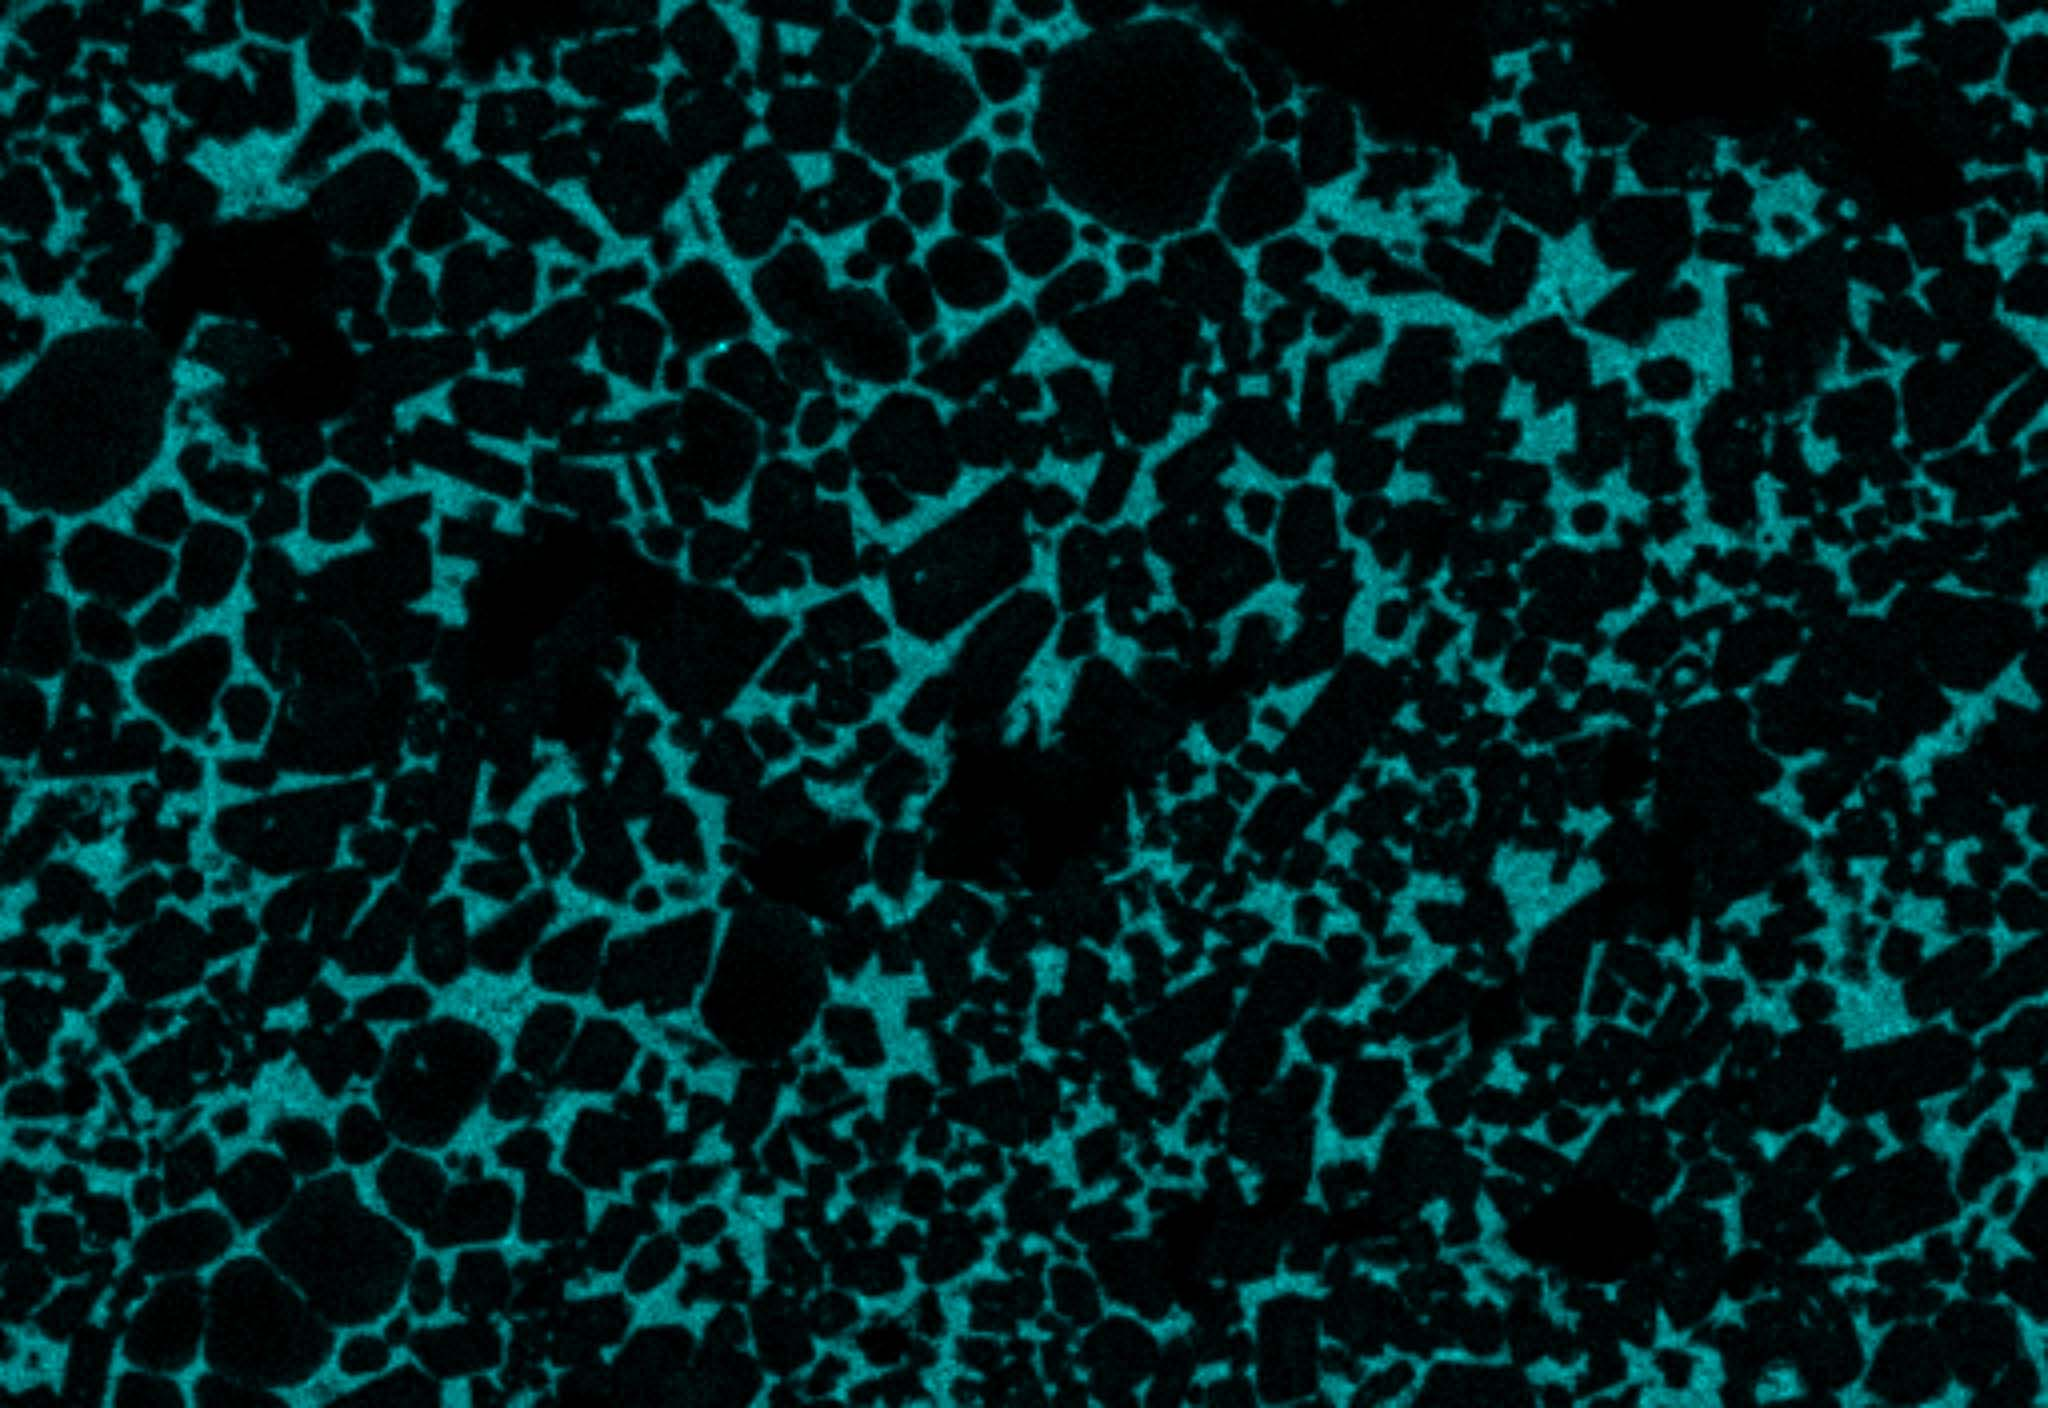
\includegraphics[width=\textwidth]{figures/la-icp-ms/edx/Al.jpg}
    \caption{Al mapping}
    \label{fig:LAICPMS-EDX-Al}
  \end{subfigure}

  \begin{subfigure}[t]{0.32\textwidth}
    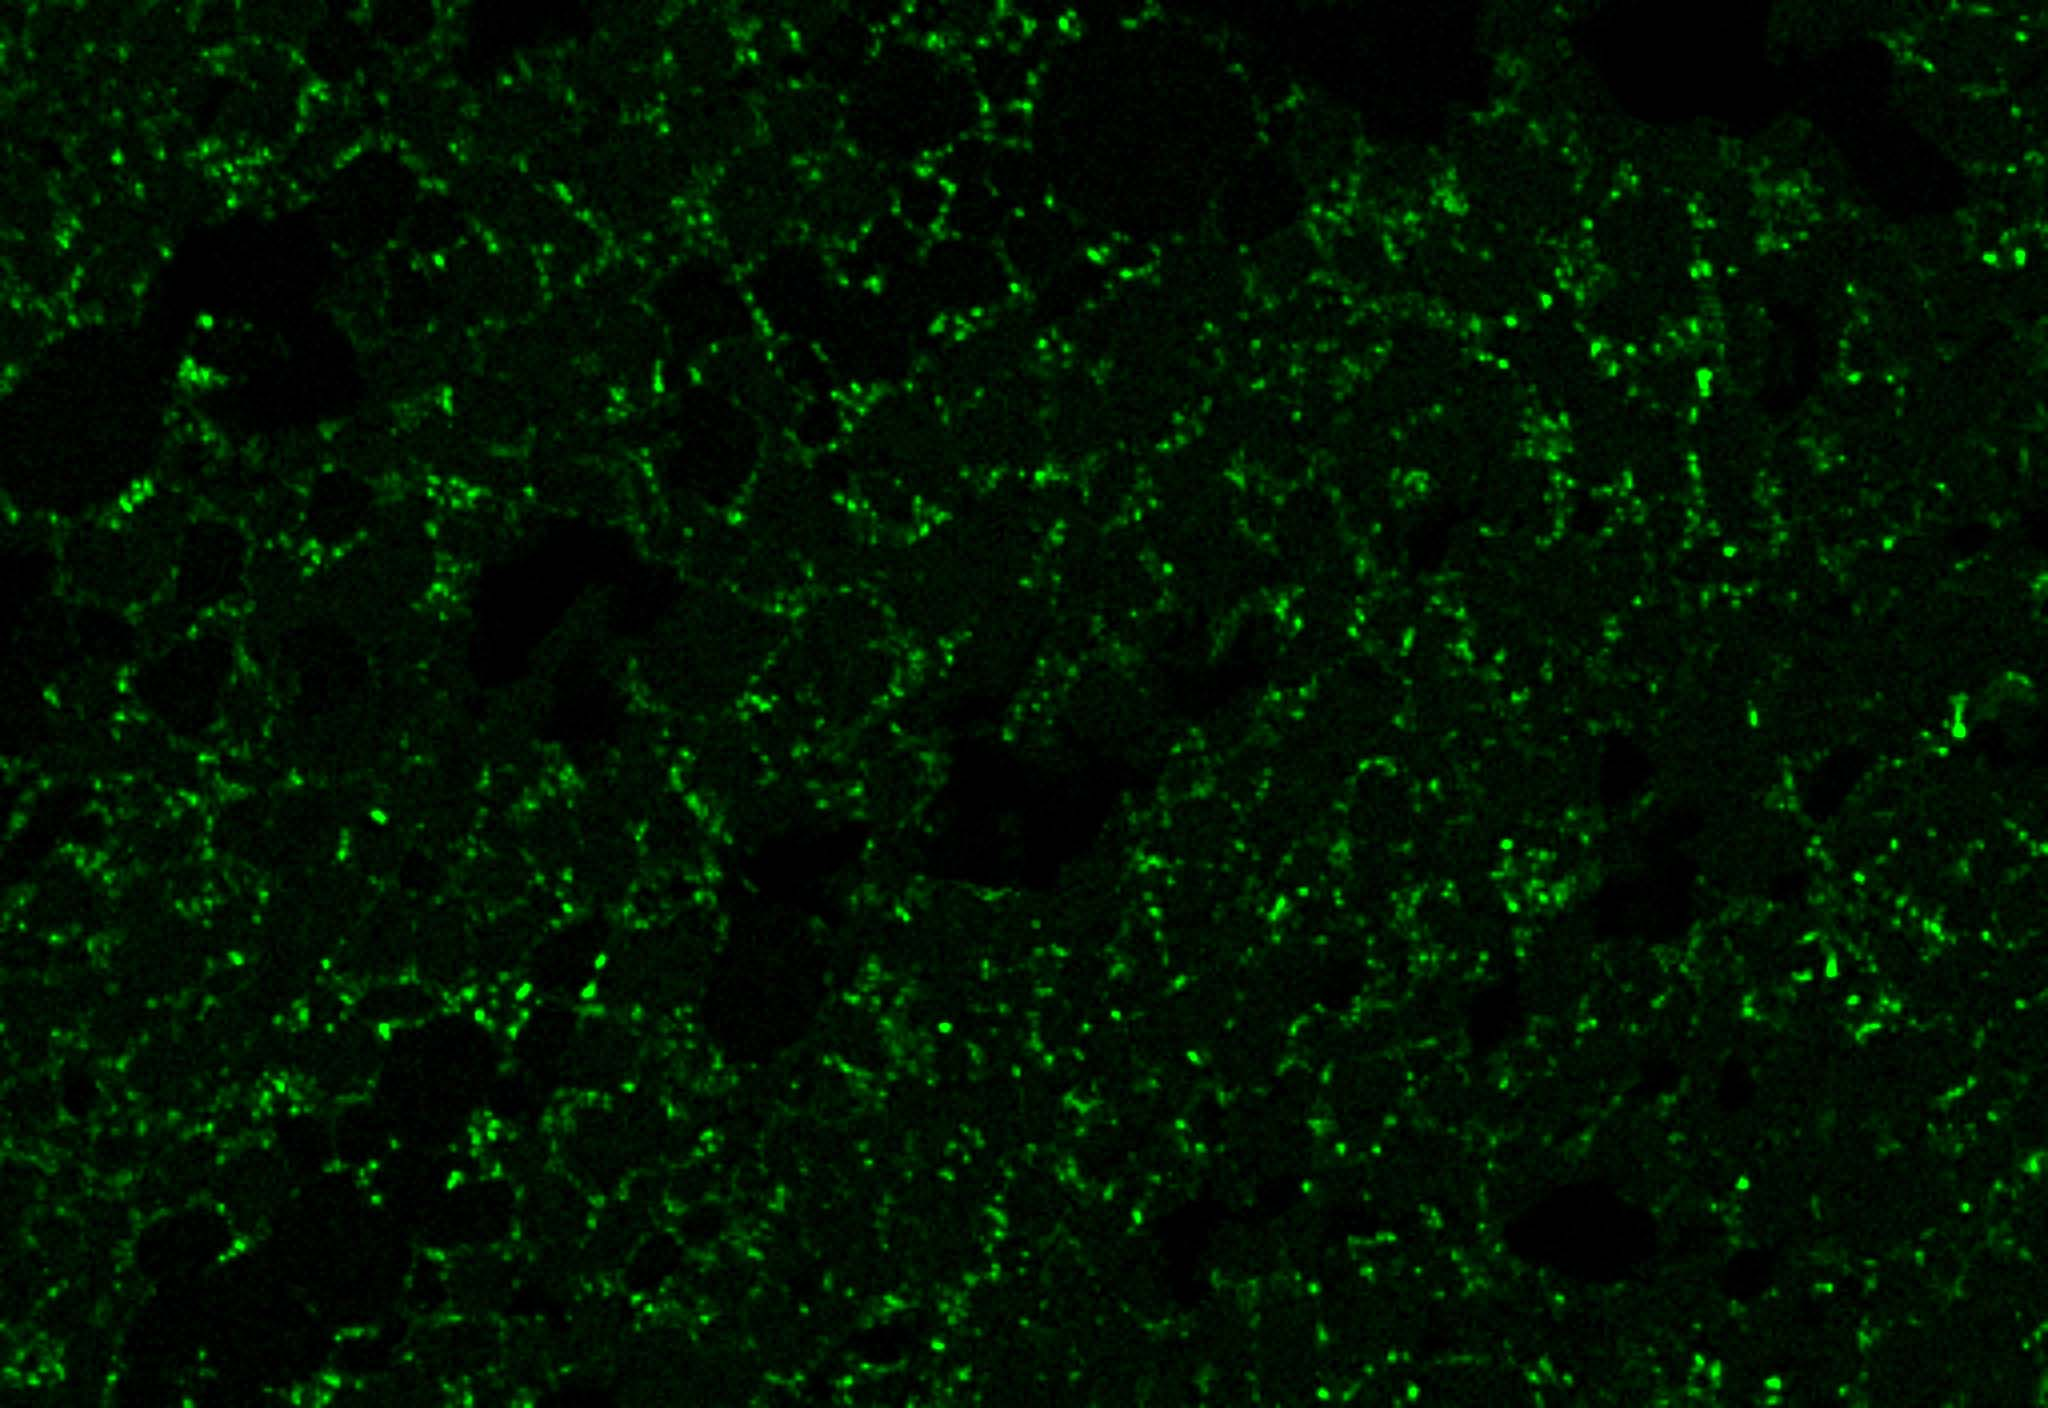
\includegraphics[width=\textwidth]{figures/la-icp-ms/edx/Mg.jpg}
    \caption{Mg mapping}
    \label{fig:LAICPMS-EDX-Mg}
  \end{subfigure}
  \hfill
  \begin{subfigure}[t]{0.32\textwidth}
    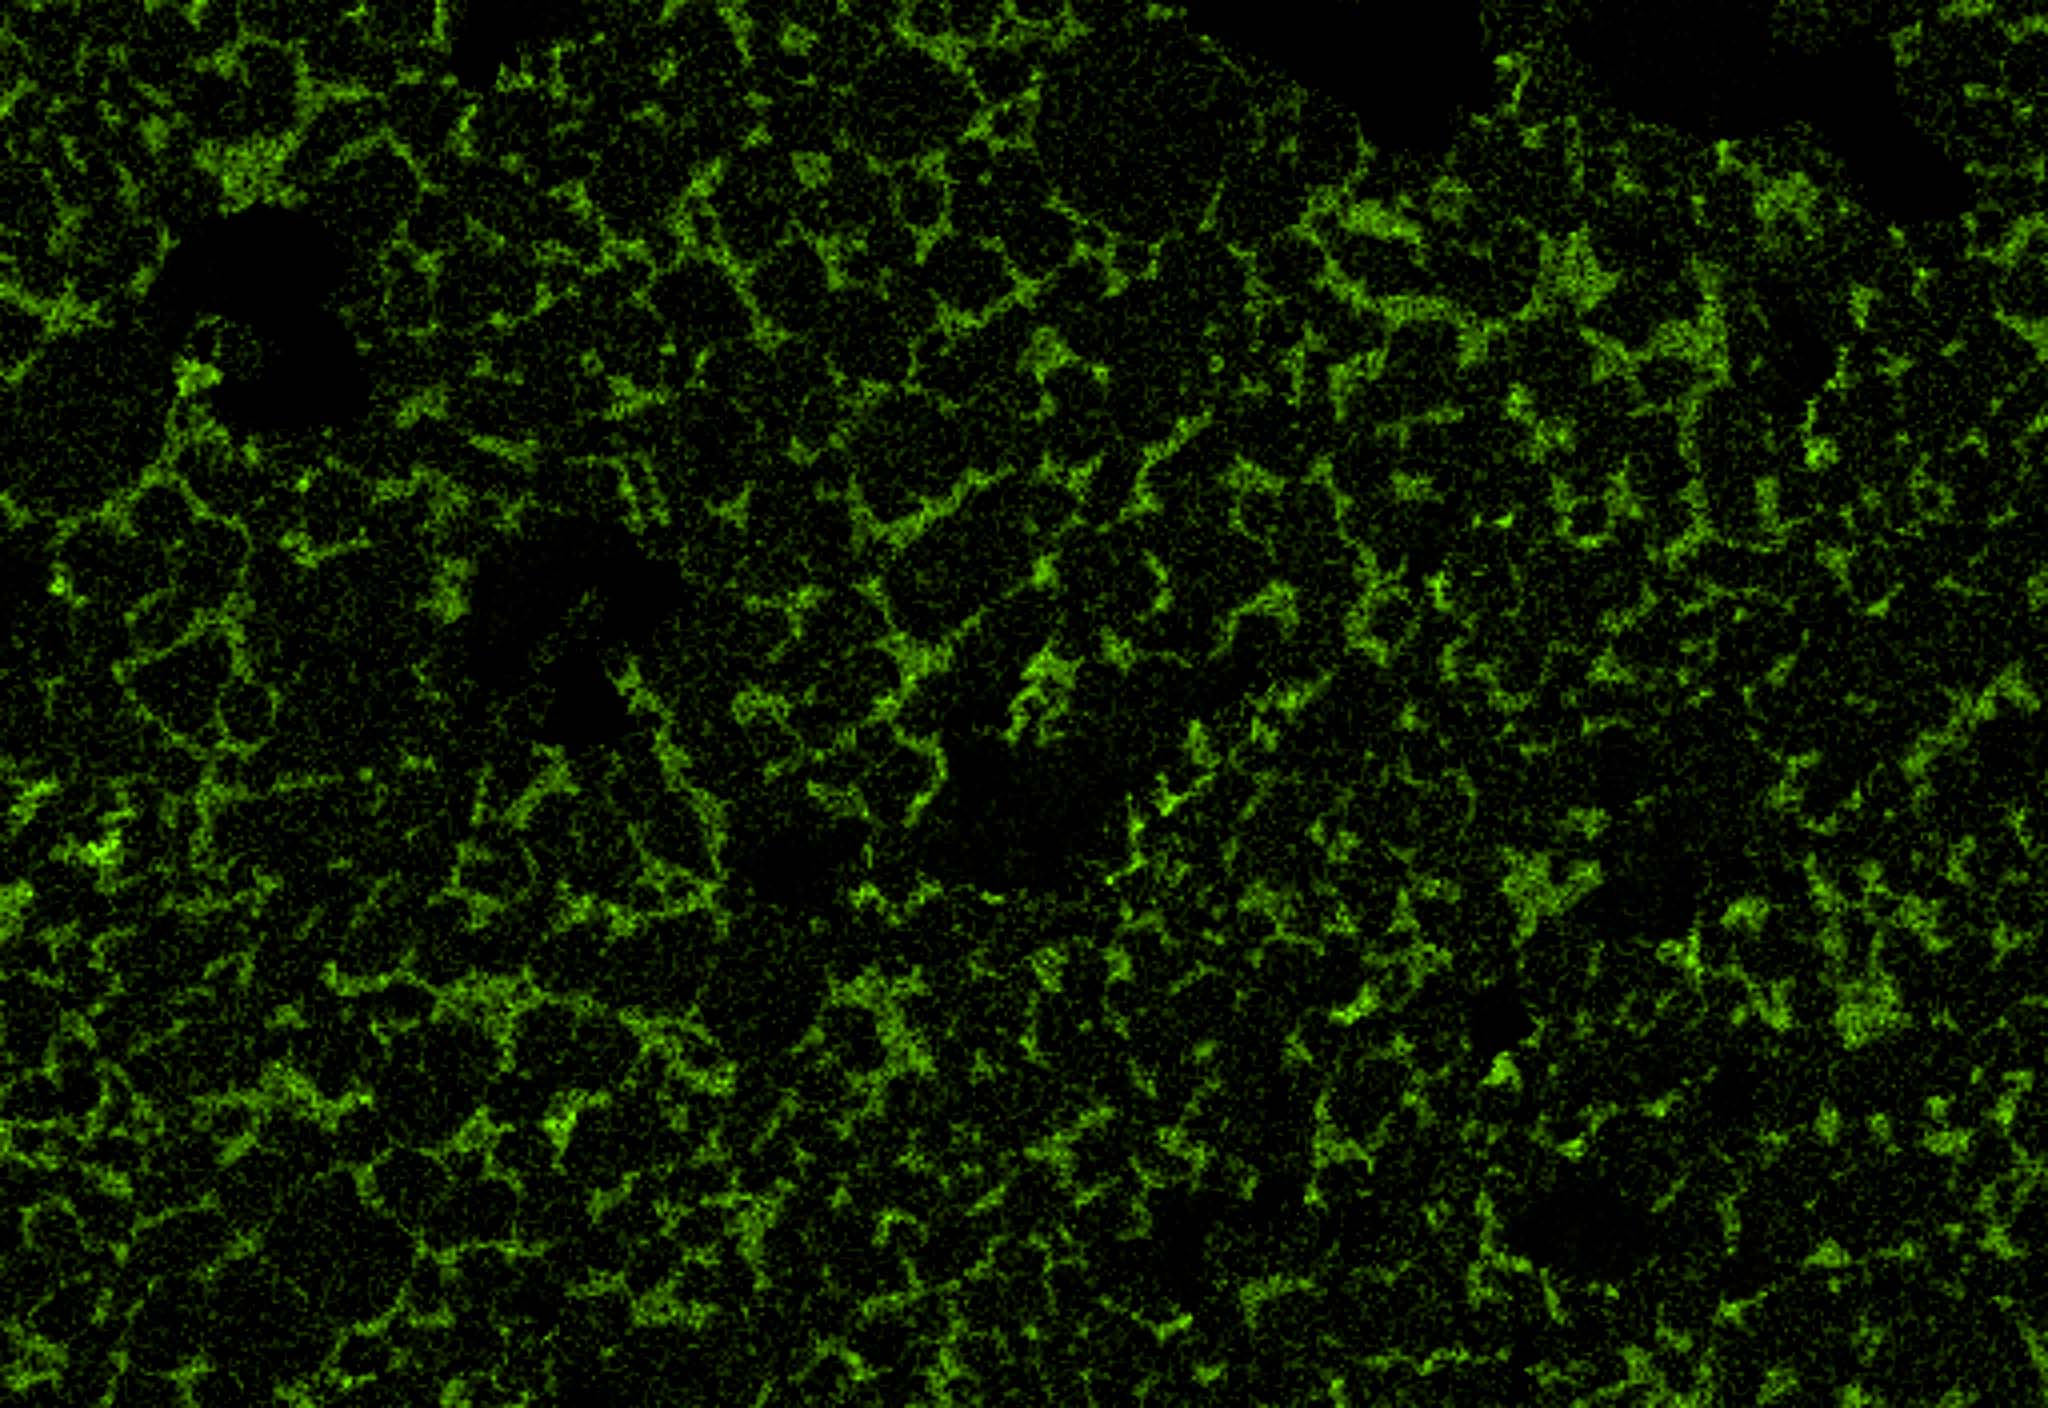
\includegraphics[width=\textwidth]{figures/la-icp-ms/edx/Fe.jpg}
    \caption{Fe mapping}
    \label{fig:LAICPMS-EDX-Fe}
  \end{subfigure}
  \hfill
  \begin{subfigure}[t]{0.32\textwidth}
    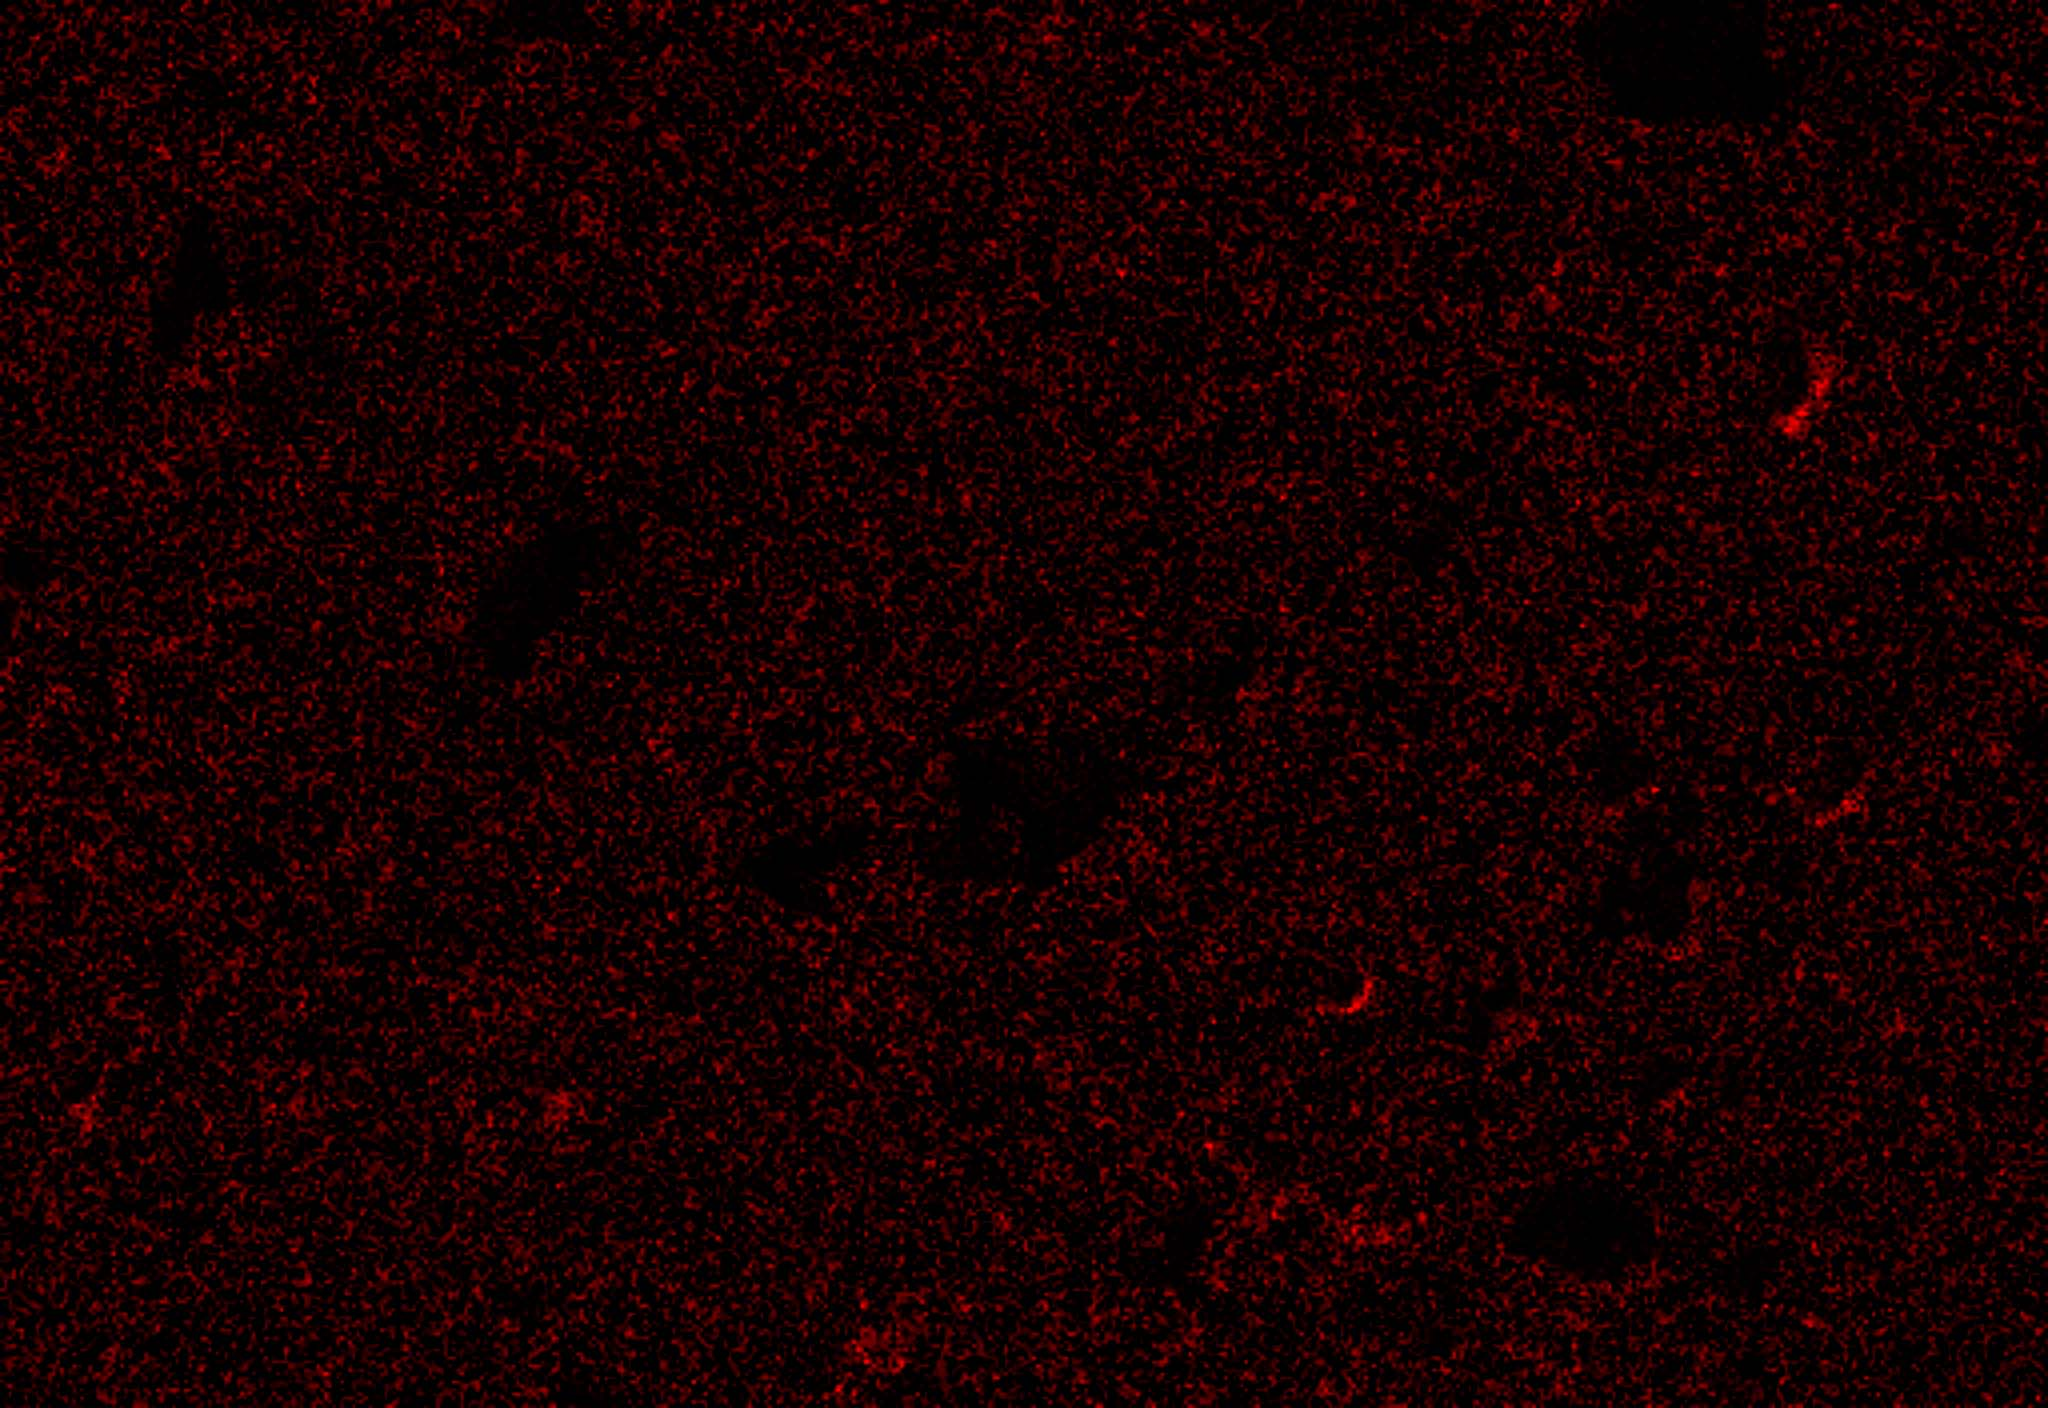
\includegraphics[width=\textwidth]{figures/la-icp-ms/edx/Na.jpg}
    \caption{Na mapping}
    \label{fig:LAICPMS-EDX-Na}
  \end{subfigure}

  \begin{subfigure}[t]{0.32\textwidth}
    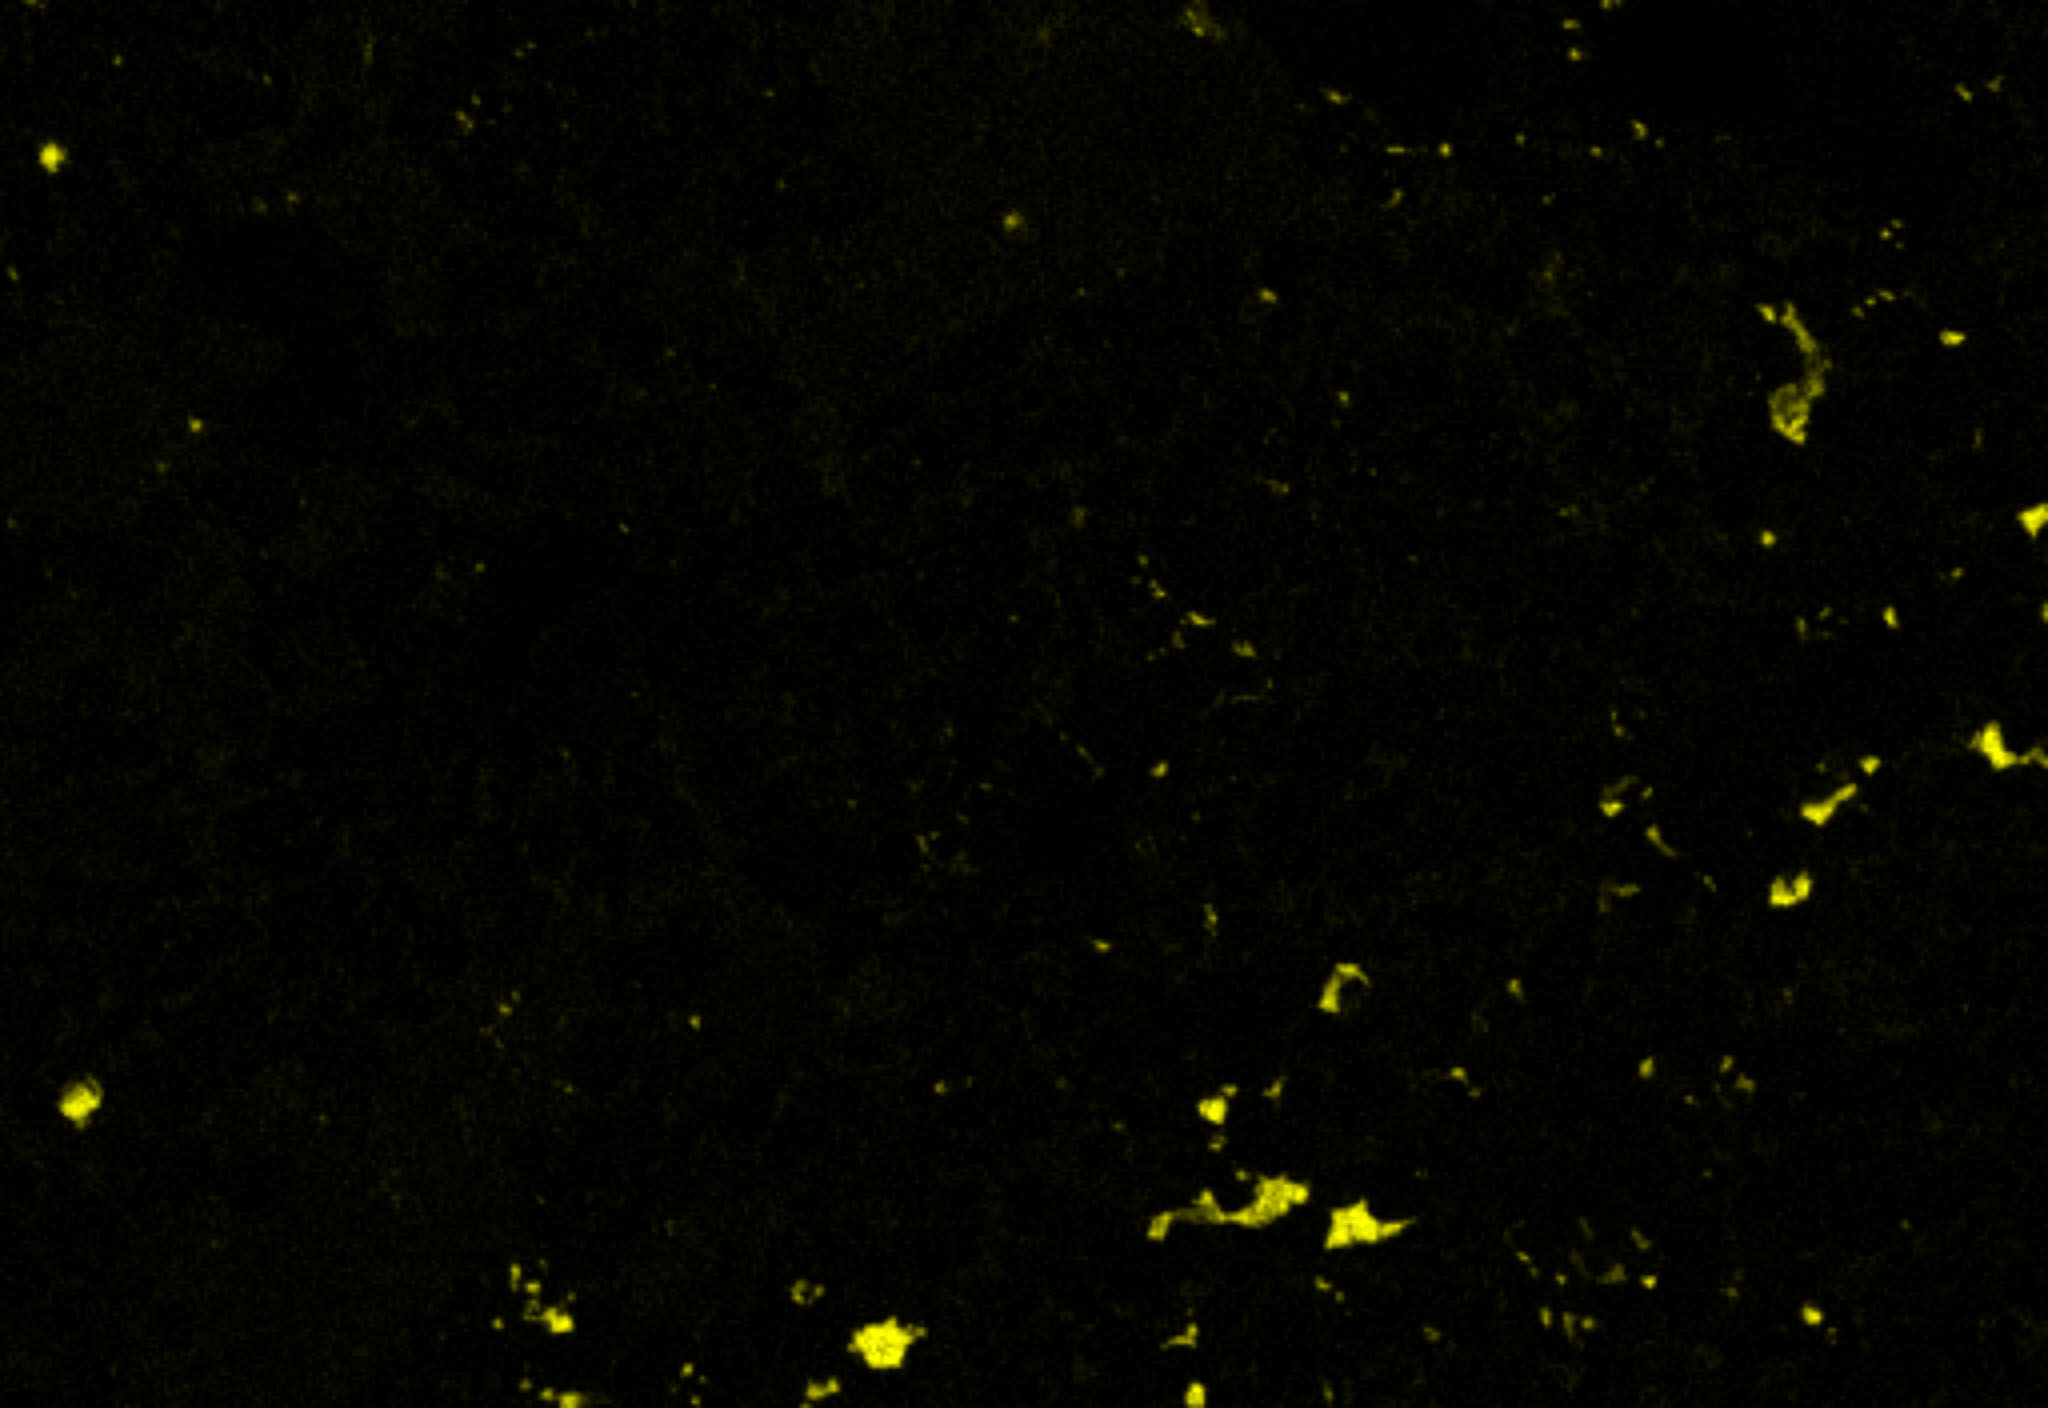
\includegraphics[width=\textwidth]{figures/la-icp-ms/edx/K.jpg}
    \caption{K mapping}
    \label{fig:LAICPMS-EDX-K}
  \end{subfigure}
  \hfill
  \begin{subfigure}[t]{0.32\textwidth}
    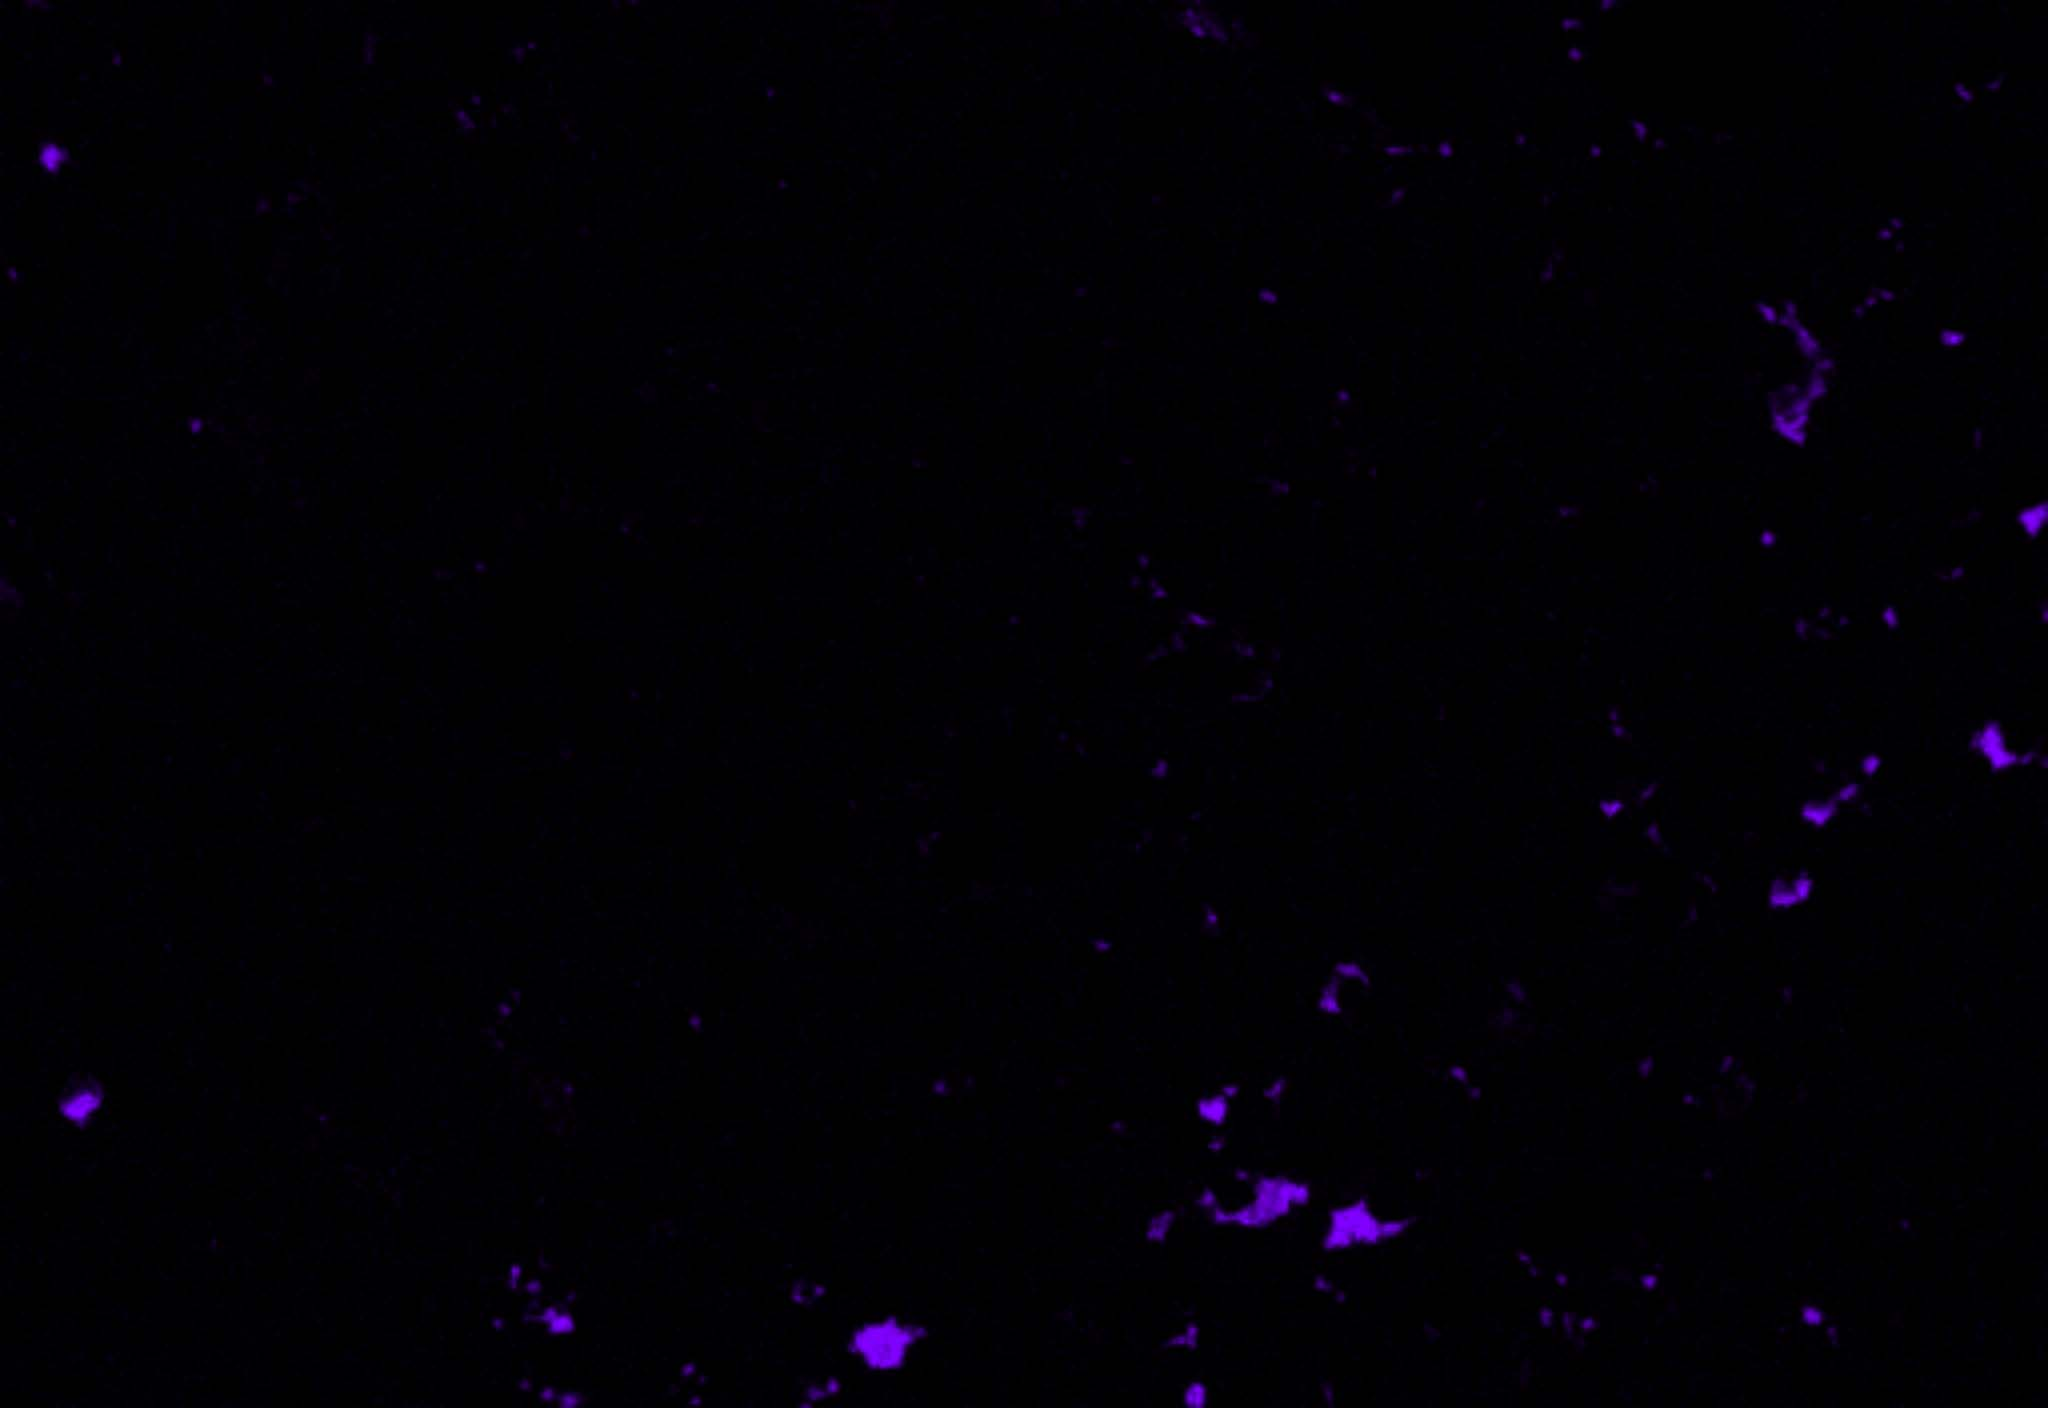
\includegraphics[width=\textwidth]{figures/la-icp-ms/edx/S.jpg}
    \caption{S mapping}
    \label{fig:LAICPMS-EDX-S}
  \end{subfigure}
  \hfill
  \begin{subfigure}[t]{0.32\textwidth}
    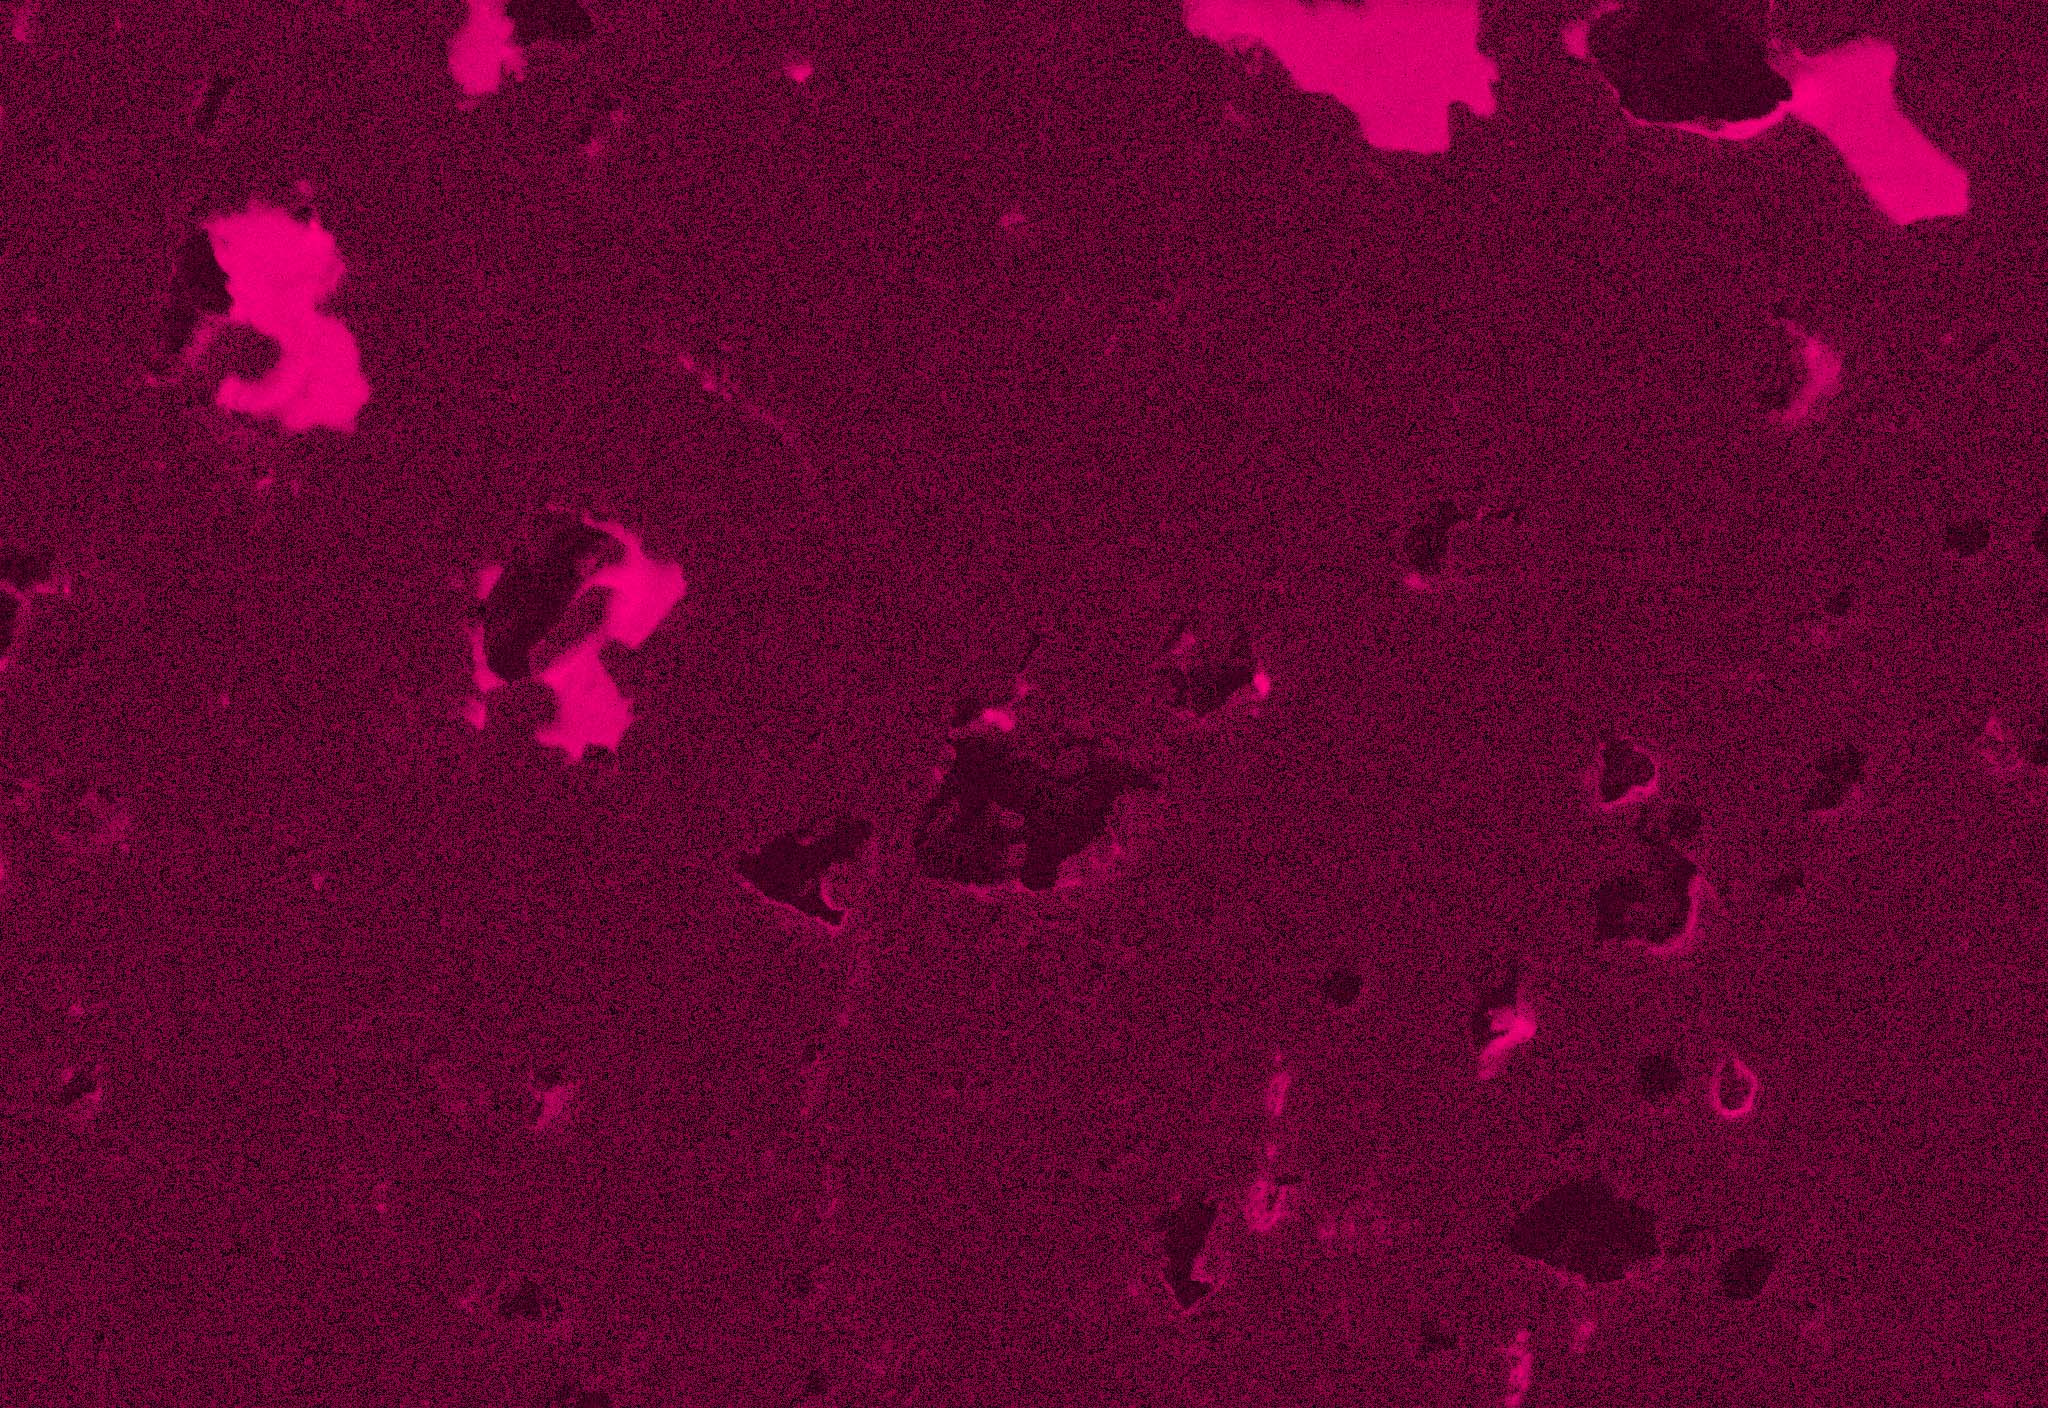
\includegraphics[width=\textwidth]{figures/la-icp-ms/edx/C.jpg}
    \caption{C mapping (epoxy resin)}
    \label{fig:LAICPMS-EDX-C}
  \end{subfigure}

  \caption{
    Element distribution maps of \ce{Ca}, \ce{Si}, \ce{Al}, \ce{Mg}, \ce{Fe}, \ce{Na}, \ce{K}, \ce{S}, and \ce{C}  of the example area.
    The images have a dimension of \qtyproduct{414 x 285}{\micro\meter\squared}.
    Data published in the \ac{SI} in \cite{kleiner.2022b}.
  }
  \label{fig:LAICPMS-EDX}
\end{figure}

A full phase map was calculated using the software Aztec 5.0 and the result is shown in \zcref{fig:LAICPMS-phasemap}.
The comparison with the \ce{Si} element distribution map in \zcref{fig:LAICPMS-EDX-Si} reveals that the phase map distinguishes \ac{C3S}, \ac{C2S}, \ce{MgO} and alkali sulphates quite well.
\ac{C3A} and \ac{C4AF} are difficult to differentiate within the \ac{LAICPMS} dataset and are therefore combined and called `interstitial phase' from here on (marked red in \zcref{fig:LAICPMS-phasemap}).

%\begin{wrapfigure}{R}{0.6\linewidth}
\begin{figure}[htb!]
  \centering
  %\vspace{-\intextsep}
  \includegraphics[width=.9\linewidth]{la-icp-ms/EDX-phase-map.pdf}
  \caption{Phase map based on the \ac{EDX}-dataset (see \zcref{fig:LAICPMS-EDX}). \cite{kleiner.2022b}, \ac{SI}}
  \label{fig:LAICPMS-phasemap}
  %\vspace{-\intextsep}
\end{figure}
%\end{wrapfigure}

The \ac{C2S} can be seen mainly on the left half of the image in three clusters containing less \ce{Ca} and more \ce{Si} than the \ac{C3S}.
The \ce{Al}-rich interstitial phases can best be seen in the \ac{EDX} mappings, while they usually appear as light (\ac{C4AF}) to medium grey (\ac{C3A}) in the \ac{BSE} image between the \ac{C3S} crystals.

The positions of the minor phases \ce{K2SO4} and \ce{MgO} are indicated by the \ce{Mg} and \ce{S} distributions (\zcref{fig:LAICPMS-EDX-Mg} and \zcref{fig:LAICPMS-EDX-S}).
However, the \ce{MgO} phase positions are not visible in the phase map, due to their small size.
Elements like \ce{C} and \ce{Cl} cannot be considered for further analysis, since they are contained in the epoxy resin.
%In contrast, the maps of \ce{Na} and \ce{Ti} are very noisy and difficult to interpret.
%These mappings can be found in Figure~S-2.

%At least for unhydrated clinker, the individual phases seemed to be damaged in a similar fashion, while the epoxy resin was ablated a lot deeper.

The signal of other elements like \ce{Ti}, \ce{Cr}, \ce{Cu}, \ce{Mn} and \ce{P} was too low to generate useful element distribution maps.
Generally, elemental maps can be obtained in good quality if the X-ray count of the respective mappings is increased by increasing the measurement time.
However, the \ac{EDX} quality was not the major focus of this study.

\begin{figure}[!htb]
  \centering
  \begin{tikzpicture}
    \begin{semilogyaxis}[
        xtick = data,
        symbolic x coords={Ca,Si,Al,Fe,Mg,K,S,Na,Ti,P,Mn,Cr},
        table/col sep=comma,
        log origin=infty,
        width=\textwidth,
        height=7cm,
        ybar,
        bar width=8pt,
        enlarge x limits=0.07,
        ylabel={concentration in \unit{\wtpercent}},
        ytick={0.01,0.1,1,10,100},
        yticklabels={0.01,0.1,1,10,100},
        ymin=0.008, ymax=100,
        legend cell align=left,
        legend style={
            at={(0.98,0.97)},
            anchor=north east,
            column sep=4pt
        },
        legend columns=-1,
        error bars/y dir=both,
        error bars/y explicit,
        scaled y ticks = false,
        error bars/y dir=both,
        error bars/y explicit,
    ]

      \addplot[
        darkgreen,fill=darkgreen,
      ] table [
        x=element,
        y=c_analy_alt,
        col sep=comma
      ] {figures/la-icp-ms/chemical-edx.csv};
      \addlegendentry{\acs*{ICP}-\acs*{OES} analysis};

      \addplot[
        red, fill=red,
        error bars/.cd,
        error bar style={black},
      ] table [
        x=element,
        y=EDX_mean_area,
        y error=stabw_edx_area,
        col sep=comma
      ] {figures/la-icp-ms/chemical-edx.csv};
      \addlegendentry{\ac*{EDX} analysis};

      \draw [darkred, thick, dashed] (axis cs:Ca, 0.1) node [below, anchor=north west, align=left, text=black, fill=white, fill opacity=0.7, text opacity=1] {below the \ac{EDX} detection limit} -- (axis cs:Cr, 0.1) ;

    \end{semilogyaxis}
  \end{tikzpicture}
  \caption{
    Comparison of the results (oxide concentrations) from the chemical analysis (\ac{ICP}-\ac{OES}; see \zcref{tab:laicpms-clinker}) and the \ac{EDX} analysis obtained from the sum spectra of the three mappings.
    \cite{kleiner.2022b}
  }
  \label{fig:LAICPMS-EDX-chemical}
\end{figure}

To validate the \ac{EDX} results, they were compared to the \ac{ICP}-\ac{OES} measurement (see \zcref{tab:laicpms-clinker}).
For this purpose, the \ac{EDX} results were averaged over the three mappings and the results were plotted in \zcref{fig:LAICPMS-EDX-chemical}.
However, the \ac{ICP}-\ac{OES} results are mostly within the range of the \ac{EDX} standard deviations.
The concentrations of \ce{S} and \ce{Mg} and other low concentrated elements show obvious differences.
This indicates that the area analysed using \ac{EDX} is too small to be representative to obtain a chemical composition close to the \ac{ICP}-\ac{OES} results.
Concentrations below \qty{0.1}{\wtpercent} oxide are outside the \ac{EDX} detection limit — this concerns the elements \ce{Na}, \ce{P}, \ce{Mn} and \ce{Cr}.
%TODO: MIB: Das "EDX detection limit" ist irgendwie seltsam, weil du ja dann trotzdem Elemente wie P, Mn, Cr mit verhältnismäßig kleinem Fehlerbalken angibst.
% Das Detektionslimit ist doch sicherlich auch vom Element abhängig oder? Du hast ja hier die "Konzentration" in wg.-% angegeben, wie kommt man da überhaupt auf ein Limit von 0.1 wt.-%. Die Masse des Elements spielt hier doch auch eine Rolle.
\begin{figure}[htb!]
  \centering

  \ifdefined\PRINTABLE
    \includegraphics[width=\textwidth]{la-icp-ms/la-icp-ms-mapping/result0.pdf}
  \else
    \animategraphics[loop,autoplay,width=\textwidth]{1}{la-icp-ms/la-icp-ms-mapping/result}{0}{2}
  \fi

  \caption{
    Element distribution maps generated by \ac{LAICPMS}.
    The images cover an area of \qtyproduct{483.8 x 343.4}{\micro\meter\squared} using \numproduct{80 x 603} measurements.
    The colorbars are normalised to the maximum concentration of each element (in \unit{\wtpercent} oxide).
    The outlines for \ac{C3S} (black) and \ac{C2S} (white) were derived from the \ac{EDX}-phase map shown in \zcref{fig:LAICPMS-phasemap}. \ac{SI} in \cite{kleiner.2022b}
  }
  \label{fig:LAICPMS-la-maps}
\end{figure}

Results in \zcref{fig:LAICPMS-la-maps} show the element distribution maps obtained by \ac{LAICPMS}.
Some elements show regions of very high concentrations, which will be called hotspots from hereon.
A comparison of the \ce{Al} element distribution maps obtained by both methods (\zcref{fig:LAICPMS-EDX, fig:LAICPMS-la-maps}) reveals that \ac{LAICPMS} does not distinctly resolve the phase boundaries between the finely grained interstitial phases (\ac{C3A} and \ac{C4AF}) and the silicate phases.
This limitation becomes particularly apparent when the size of the laser ablation spot exceeds that of the individual phases, such as \ac{C3A} and \ac{C4AF}.
By combining phase segmentation based on the \ac{EDX} maps with the \ac{LAICPMS} data (\zcref{fig:LAICPMS-la-maps}), the relevant phases (\ac{C3S}, \ac{C2S}, \ac{C4AF}, and \ac{C3A}) can be analysed in detail.
A comparison of the quantification results obtained by \ac{EDX} and \ac{LAICPMS} for the interstitial phase is presented in \zcref{fig:LAICPMS-la-maps, fig:LA-EDX-results-high, fig:LA-EDX-results-low}.

The \ce{Al} content measured by \ac{EDX} and \ac{LAICPMS} at identical locations exhibits considerable variation (\zcref{fig:LA-EDX-results-low}).
For example, \ac{EDX} yielded a concentration of \qty{23.1}{\wtpercent}, whereas \ac{LAICPMS} measured \qty{7.8(4.2)}{\wtpercent}.
The observed discrepancy may be attributed to several factors, including potential inaccuracies in dataset registration, calibration errors, or, most plausibly, phase heterogeneity caused by differences in the depth of signal generation.
Nevertheless, the concentrations determined for \ce{Al}, \ce{Mg}, \ce{Ti}, \ce{K}, \ce{Na}, and \ce{Mn} (\zcref{fig:LA-EDX-results-high, fig:LA-EDX-results-low}) consistently remain within the same order of magnitude.
These findings proof that the laser spot size (\qtyproduct{6x6}{\micro\meter\squared}) is too large to quantitatively analyse the interstitial phases.
Nevertheless, enrichment of for example \ce{Mn} in the interstitial phase can be proven by \ac{LAICPMS}.
Furthermore, an inaccurate image registration seems to be a minor problem, as the same trends in major, minor and trace element concentration can be found in all investigated areas (compare \zcref{tab:laicpms1-area1, tab:laicpms2-area1,tab:laicpms1-area2, tab:laicpms2-area2,tab:laicpms1-area3, tab:laicpms2-area3}, as in the \ac{SI} from \cite{kleiner.2022b}).

\begin{figure}[!htb]
  \centering

  % Subfigure 1: Alite
  \begin{subfigure}[b]{0.36\textwidth}
    \begin{tikzpicture}
      \begin{semilogyaxis}[
          xtick=data,
          symbolic x coords={Al,Mg,K,Na,Ti},
          ytick={0.001,0.01,0.1,1,10},
          yticklabels={0.001,0.01,0.1,1,10},
          xticklabel style={font=\footnotesize},
          yticklabel style={font=\footnotesize},
          table/col sep=comma,
          width=1.05\textwidth,
          height=6cm,
          log origin=infty,
          ybar,
          bar width=5pt,
          enlarge x limits=0.15,
          ylabel={concentration in \unit{\percent}},
          ymin=0.008, ymax=40,
          error bars/y dir=both,
          error bars/y explicit,
          scaled y ticks = false,
      ]
        \addplot[
          cyan,fill=cyan,
          error bars/.cd,
          error bar style={black},
        ] table [
          x=Isotope,
          y=La_map_c_C3S,
          y error=La_map_err_C3S,
          col sep=comma
        ] {figures/la-icp-ms/element_analysis_EDX_La.csv};

        \addplot[
          red,fill=red,
          error bars/.cd,
          error bar style={black},
        ] table [
          x=Isotope,
          y=EDX_map_c_C3S,
          y error=EDX_map_err_C3S,
          col sep=comma
        ] {figures/la-icp-ms/element_analysis_EDX_La.csv};

        \draw [darkred, thick, dashed] (axis cs:Al, 0.1) -- (axis cs:Ti, 0.1);
        \node[above, font=\footnotesize, xshift=-4pt] at (axis cs:K, 2) {*};

      \end{semilogyaxis}
    \end{tikzpicture}
    \caption{\ac{C3S}}
    \label{fig:LA-EDX-results-alite}
  \end{subfigure}
  \hfill
  % Subfigure 2: Belite
  \begin{subfigure}[b]{0.30\textwidth}
    \begin{tikzpicture}
      \begin{semilogyaxis}[
          xtick=data,
          symbolic x coords={Al,Mg,K,Na,Ti},
          ytick={0.001,0.01,0.1,1,10},
          yticklabels={}, % Remove y tick labels
          xticklabel style={font=\footnotesize},
          table/col sep=comma,
          width=1.27\textwidth,
          height=6cm,
          log origin=infty,
          ybar,
          bar width=5pt,
          enlarge x limits=0.15,
          ylabel={}, % Remove y label
          ymin=0.008, ymax=40,
          legend cell align=center,
          legend style={
              at={(0.5,0.99)},
              anchor=north,
              column sep=4pt,
              font=\footnotesize
          },
          legend columns=-1,
          error bars/y dir=both,
          error bars/y explicit,
          scaled y ticks = false,
      ]
        \addplot[
          cyan,fill=cyan,
          error bars/.cd,
          error bar style={black},
        ] table [
          x=Isotope,
          y=La_map_c_C2S,
          y error=La_map_err_C2S,
          col sep=comma
        ] {figures/la-icp-ms/element_analysis_EDX_La.csv};
        \addlegendentry{\ac{LAICPMS}};

        \addplot[
          red,fill=red,
          error bars/.cd,
          error bar style={black},
        ] table [
          x=Isotope,
          y=EDX_map_c_C2S,
          y error=EDX_map_err_C2S,
          col sep=comma
        ] {figures/la-icp-ms/element_analysis_EDX_La.csv};
        \addlegendentry{\ac{EDX}};

        \draw [darkred, thick, dashed] (axis cs:Al, 0.1) -- (axis cs:Ti, 0.1);

      \end{semilogyaxis}
    \end{tikzpicture}
    \caption{\ac{C2S}}
    \label{fig:LA-EDX-results-belite}
  \end{subfigure}
  \hfill
  % Subfigure 3: C4AF
  \begin{subfigure}[b]{0.30\textwidth}
    \begin{tikzpicture}
      \begin{semilogyaxis}[
          xtick=data,
          symbolic x coords={Al,Mg,K,Na,Ti},
          ytick={0.001,0.01,0.1,1,10},
          yticklabels={},%{0.001,0.01,0.1,1,10},
          xticklabel style={font=\footnotesize},
          table/col sep=comma,
          width=1.27\textwidth,
          height=6cm,
          log origin=infty,
          ybar,
          bar width=5pt,
          enlarge x limits=0.15,
          ylabel={},%{Difference to mean concentration in \unit{\percent}},
          ymin=0.008, ymax=40,
          error bars/y dir=both,
          error bars/y explicit,
          scaled y ticks = false,
          yticklabel pos=right,
      ]
        \addplot[
          cyan,fill=cyan,
          error bars/.cd,
          error bar style={black},
        ] table [
          x=Isotope,
          y=La_map_c_C4AF,
          y error=La_map_err_C4AF,
          col sep=comma
        ] {figures/la-icp-ms/element_analysis_EDX_La.csv};

        \addplot[
          red,fill=red,
          error bars/.cd,
          error bar style={black},
        ] table [
          x=Isotope,
          y=EDX_map_c_C4AF,
          y error=EDX_map_err_C4AF,
          col sep=comma
        ] {figures/la-icp-ms/element_analysis_EDX_La.csv};

        \draw [darkred, thick, dashed] (axis cs:Al, 0.1) -- (axis cs:Ti, 0.1);
        \node[above, font=\footnotesize, xshift=-4pt] at (axis cs:K, 2) {*};

      \end{semilogyaxis}
    \end{tikzpicture}
    \caption{interstitial phase}
    \label{fig:LA-EDX-results-C4AF}
  \end{subfigure}

  \caption{
    Mean main element concentrations for \ac{C3S}, \ac{C2S} and the interstitial phase, determined by segmented \ac{LAICPMS} mappings.
    The \ac{EDX} detection limit of \qty{0.1}{\wtpercent} is marked as dashed line.
    Bars marked with an asterisk (*) have a standard deviation exceeding the $x$-axis.
    Therefore only the upper value is marked.
    Based on \cite{kleiner.2022b}
  }
  \label{fig:LA-EDX-results-high}
\end{figure}

%\begin{wrapfigure}{R}{0.6\linewidth}
\begin{figure}[!htb]
  \centering
  \begin{tikzpicture}
    \begin{semilogyaxis}[
        xtick=data,
        symbolic x coords={Mn,Zn,Ba,Cr,V,Rb},
        ytick={0.001,0.01,0.1,1},
        yticklabels={0.001,0.01,0.1,1},
        xticklabel style={font=\footnotesize},
        yticklabel style={font=\footnotesize},
        table/col sep=comma,
        width=.7\linewidth,
        height=6cm,
        log origin=infty,
        ybar,
        bar width=7pt,
        enlarge x limits=0.15,
        ylabel={concentration in \unit{\percent}},
        ymin=0.001, ymax=.3,
        error bars/y dir=both,
        error bars/y explicit,
        scaled y ticks = false,
        legend cell align=left,
        legend columns = 1,
        legend style={
            at={(1.03,0.5)},
            anchor=west,
            column sep=4pt
        },
    ]
    \addplot[
      orange,fill=orange,
      error bars/.cd,
      error bar style={black},
    ] table [
      x=Isotope,
      y=La_map_c_C3S,
      y error=La_map_err_C3S,
      col sep=comma
    ] {figures/la-icp-ms/element_analysis_LA.csv};

    \addplot[
      red,fill=red,
      error bars/.cd,
      error bar style={black},
    ] table [
      x=Isotope,
      y=La_map_c_C2S,
      y error=La_map_err_C2S,
      col sep=comma
    ] {figures/la-icp-ms/element_analysis_LA.csv};

    \addplot[
      blue,fill=blue,
      error bars/.cd,
      error bar style={black},
    ] table [
      x=Isotope,
      y=La_map_c_C4AF,
      y error=La_map_err_C4AF,
      col sep=comma
    ] {figures/la-icp-ms/element_analysis_LA.csv};

    \addlegendentry{\ac{C3S}};
    \addlegendentry{\ac{C2S}};
    \addlegendentry{interstitial phase};


    \node[above, font=\footnotesize, xshift=-9pt] at (axis cs:Zn, 0.08) {*};
    \node[above, font=\footnotesize] at (axis cs:Zn, 0.075) {*};
    \node[above, font=\footnotesize, xshift=+9pt] at (axis cs:Zn, 0.08) {*};

    \node[above, font=\footnotesize, xshift=-9pt] at (axis cs:Ba, 0.05) {*};
    \node[above, font=\footnotesize, xshift=+9pt] at (axis cs:Ba, 0.05) {*};

    \node[above, font=\footnotesize, xshift=-9pt] at (axis cs:Cr, 0.02) {*};
    \node[above, font=\footnotesize] at (axis cs:Cr, 0.017) {*};
    \node[above, font=\footnotesize, xshift=+9pt] at (axis cs:Cr, 0.02) {*};

    \end{semilogyaxis}
  \end{tikzpicture}

  \caption{
    Mean trace element concentrations for \ac{C3S}, \ac{C2S} and the interstitial phase, determined by segmented \ac{LAICPMS} mappings.
    Bars marked with an asterisk (*) have a standard deviation exceeding the $x$-axis.
    Therefore, only the upper value is marked.
    Based on \cite{kleiner.2022b}
  }
  \label{fig:LA-EDX-results-low}
  %\vspace{-\intextsep}
\end{figure}
%\end{wrapfigure}

Differences in the distribution of trace elements between \ac{C3S} and \ac{C2S} are also visible in \zcref{fig:LAICPMS-la-maps}.
Especially the \ce{Ba}, \ce{Rb} and \ce{V} mappings show a noticeable concentration variation in both phases and are mostly enriched in \ac{C2S}.
For the interstitial phase high \ce{Al} concentrations are expected.
The mappings also reveal an accumulation of \ce{Mn}, and \ce{Ti}.

As shown by \ac{EDX} element maps (\zcref{fig:LAICPMS-EDX}), \ce{K} is associated with \ce{S} via \ce{K2SO4}.
Comparing these locations with hotspots of \ce{Rb}, \ce{Cr} and \ce{K} in the \ac{LAICPMS} measurements reveals, that these elements are mostly incorporated in \ce{K2SO4}.
\ce{V}, \ce{Zn} can also be found in higher concentrations within the \ce{K2SO4} phase, while they also occur in other phases.


%For the same area the presence of the following trace elements (i.e. <\,\qty{0.1}{\wtpercent}) could be proven by \ac{LAICPMS}: \ce{Ba}, \ce{Zn}, \ce{Cr}, \ce{V}, \ce{Rb} (\zcref{fig:LAICPMS-la-maps, LA-EDX-results-low-all, LA-EDX-results-low}).
%The quantified concentrations of \ce{Ba}, \ce{Zn}, \ce{Cr}, \ce{V}, \ce{Rb} are similar for all analysed areas ({\color{red}see supplementary document}).
%Reversely, this results in the observed low \ce{Al} concentration (\zcref{fig:LAICPMS-la-maps, LA-EDX-results-low-all} and Figure~S-22).


%% maybe omit the spot analysis part, as it is not really relevant for the main topic of the thesis
% \section{\acs*{LA-ICP-MS} spot analysis}

% In addition to \ac{LAICPMS} and \ac{EDX} mapping data, spot analyses have been collected on sites that were selected based on the \ac{EDX} element distribution maps.
% The prerequisite for selecting sites for spot analyses was that the area should be large enough to ensure that the laser spot ablates only a single phase.
% Therefore, the laser ablation spots are re-allocated on the \ac{BSE} image and the \ac{EDX} phase map (Figure~9). Obviously, the spots for belite were more successfully placed in large homogeneous areas than for alite.
% The reason is the smaller size of alite crystals.

% For the spot analysis, more elements could be measured as the signal to noise ratio is drastically increased when the spot size is enlarged from approximately \qty{36}{\micro\meter\squared} (square shape) to \qty{415}{\micro\meter\squared} (round shape).
% Thus, \ac{Pb}, \ac{Ni}, \ac{As}, \ac{Sr}, \ac{Cu} and \ac{P} could be measured additionally in the spot analysis.
% However, other trace elements like \ac{Hg} and \ac{Sb} still cannot be measured because of their extremely low concentration even if it would be possible to further enlarge the spot size to improve the detection limit.

% There are rather large deviations between mapping and spot analysis for most of the elements in alite and belite (Figure~10 and 11).
% Besides different calibration methods, another reason for this deviation is most likely the effect that during spot ablation more area from neighbouring phases is analysed than in mapping mode (larger spot size).
% Furthermore, the \ac{LAICPMS} results are further deviated due to the $z$-effect, e.g. by material that is ablated from a certain depth.
% This $z$-effect is also occurring in \ac{EDX} analysis but for the used \qty{12}{\kilo\volt} acceleration voltage the excitation volume diameter is not larger than \qtyrange{1.6}{2.0}{\micro\meter}, depending on the material. Therefore, both \ac{EDX} and \ac{LAICPMS} are often affected by neighbouring phases in 3 dimensions, if the phase size is similar or smaller than the analysed sample volume.
% Figure~10 and 11 show the quantitative element concentrations for alite and belite obtained from segmented mappings (given in \unit{\wtpercent} oxide) and from spot analyses. The following element concentrations were determined by both methods (Al, Mg, Ti, K, Na, Mn).
% The Al content in alite, as documented by results in Figure~10, as determined by \ac{SEM} -\ac{EDX} spot analysis is \qty{1.5(0.4)}{\wtpercent}, by \ac{SEM} -\ac{EDX} mapping \qty{1.5(0.0)}{\wtpercent} and by \ac{LAICPMS} mapping \qty{4.30(2.88)}{\wtpercent} respectively \ac{LAICPMS} spot analysis: \qty{2.10(0.74)}{\wtpercent}.
% The deviation between \ac{EDX} and \ac{LAICPMS} seems rather large and is probably mainly caused by the effect of neighbouring phases, e.g. more Al from interstitial phase is detected by the \ac{LAICPMS} analysis.

% However, the spot analysis resembles the results shown by the \ac{LAICPMS} -mappings, both results reveal the accumulation of trace elements in clinker phases.
% Based on the \ac{LAICPMS} mappings it was shown that alite contains more \ce{Ba}, \ce{V} and \ce{Rb}.
% This is confirmed by spot analyses for \ce{Ba} and V but not for \ce{Rb} (Figure~10 and 11).
% But standard deviation of \ce{Rb} and most other element concentrations determined by \ac{LAICPMS} is larger for alite than for belite.
% This indicates that alite concentrations are, due to smaller crystal sizes, more affected by neighbouring phases (e.g. hotspots that contain \ce{Rb} in high concentration) than belite.



The data presented in \zcref{fig:LA-EDX-results-high, fig:LA-EDX-results-low} originating from the segmented \ac{LAICPMS} measurements support the semi-quantitative visual observations documented in \zcref{fig:LAICPMS-la-maps}.
In the following, \ce{Ba} is used as an example to evaluate the data.
The element distribution maps clearly show that \ce{Ba} is predominantly enriched in \ac{C2S} (\qty{0.0351(0.0145)}{\wtpercent}) and aluminium-rich regions (\qty{0.0234(0.0139)}{\wtpercent}) , which can be identified as interstitial phases (\ac{C3A} and \ac{C4AF}) (see \zcref{fig:LAICPMS-la-maps}).
For \ac{C3S}, the determined \ce{Ba} concentrations are \qty{0.0187(0.0113)}{\wtpercent}, which is only half the concentration found in \ac{C2S}.
However, as indicated by the mapping data in \zcref{fig:LAICPMS-la-maps}, the distribution of \ce{Ba} within the interstitial phase is less homogeneous than in \ac{C2S}.
To accurately assess the incorporation of \ce{Ba} in the interstitial phase, measurements with higher spatial resolution and an improved dataset-alignment would be required.

\begin{figure}[!htb]
  \centering
  \begin{tikzpicture}
    \begin{axis}[
        xtick = data,
        symbolic x coords={Al,Mg,K,Na,Ti,Mn,V,Zn,Ba,Cr,Rb},
        table/col sep=comma,
        width=\textwidth,
        height=8cm,
        ybar,
        bar width=8pt,
        enlarge x limits=0.07,
        ylabel={diff. to mean conc. in \unit{\percent}},
        ymin=-50, ymax=110,
        legend cell align=left,
        legend style={
            at={(0.98,0.97)},
            anchor=north east,
            column sep=4pt
        },
        legend columns=-1,
        error bars/y dir=both,
        error bars/y explicit,
        scaled y ticks = false,
    ]

      \addplot[
        orange,fill=orange,
        error bars/.cd,
        error bar style={black},
      ] table [
        x=oxide,
        y=alite,
        y error=sd_alite,
        col sep=comma
      ] {figures/la-icp-ms/phase-composition-differences.csv};
      \addlegendentry{\ac{C3S}};

      \addplot[
        red,fill=red,
        error bars/.cd,
        error bar style={black},
      ] table [
        x=oxide,
        y=belite,
        y error=sd_belite,
        col sep=comma
      ] {figures/la-icp-ms/phase-composition-differences.csv};
      \addlegendentry{\ac{C2S}};

      \addplot[
        blue,fill=blue,
        error bars/.cd,
        error bar style={black},
      ] table [
        x=oxide,
        y=C4AF,
        y error=sd_C4AF,
        col sep=comma
      ] {figures/la-icp-ms/phase-composition-differences.csv};
      \addlegendentry{interstitial phase};

    \end{axis}
  \end{tikzpicture}

  \caption{
    Difference to the mean element concentration for \ac{C3S}, \ac{C2S} and the interstitial phase.
    Concentration data originate from three \ac{LAICPMS} measurements areas.
    The error bars represent the standard deviation of an element concentration within a phase.
    \cite{kleiner.2022b}
    % Segmentation was done using the respective EDX datasets.
  }
  \label{fig:LAICPMS-final-result}
\end{figure}


%The comparison of higher concentration elements presend in \ac{LAICPMS} and \ac{SEM}-\ac{EDX} datasets indicates the limitations of \ac{LAICPMS}.
%A combination of both methods should be considered if major and minor elements are of interest.
%In a second and third dataset, at a different area on the same polished clinker grain, the described method combination of \ac{LAICPMS} and \ac{SEM}-\ac{EDX} was repeated.
%All data can be found in the supplementary document.
To test the reproducibility of the LA-ICP-MS method, the measurements were repeated on two additional areas using the described phase segmentation method.
The same sample was analysed, and comparable results and trends were observed as previously described.
The findings are summarised in \zcref{fig:LAICPMS-final-result}.
This figure visualises the enrichment of elements in \ac{C3S}, \ac{C2S}, and the interstitial phase (\ac{C3A} and \ac{C4AF}).
Although \ac{C3A}, \ac{C4AF}, and other minor phases could not be reliably distinguished and segmented in all datasets, the enrichment of \ce{Cr} and \ce{Rb} in the water-soluble \ce{K2SO4} remains evident in the presented measurement area.

\section{Conclusion}

Correlative microscopy serves as a powerful approach for the comprehensive characterisation of heterogeneous materials, bridging the gap between high spatial resolution and high analytical sensitivity.
The combination of \ac{SEM}-\ac{BSE}, \ac{EDX}, and \ac{LAICPMS} successfully demonstrated that trace elements are not uniformly distributed but preferentially incorporated into specific clinker phases.
While \ac{SEM}-\ac{EDX} provided the necessary basis for an accurate phase segmentation, \ac{LAICPMS} delivered complementary trace element data.
It revealed, for instance, the enrichment of the trace elements \ce{Ba}, \ce{V}, and \ce{Rb} in \ac{C2S}, while \ac{C3S} crystallised with a comparably low trace element content.
Despite inherent challenges related to differing interaction volumes and image registration, this multi-modal methodology offers insights into the chemical mineralogy of cement clinker that cannot be achieved with one of the methods alone.
